% vim: set ft=plaintex:

\documentclass[]{article}

\usepackage[margin=1in]{geometry}
\usepackage{fancyhdr}
\pagestyle{fancy}

\usepackage{amsmath}
\usepackage{mathtools}
\usepackage{amsfonts}
\usepackage{amssymb}
\usepackage{bbm}

\usepackage{braket}
\usepackage[bold]{hhtensor}
\usepackage{cancel}

\usepackage{amsthm}

% load thmtools but fix "proof proof" bug with thmbox
\usepackage{letltxmacro}
\LetLtxMacro\amsproof\proof
\LetLtxMacro\amsendproof\endproof

\usepackage{thmtools}

\AtBeginDocument{%
  \LetLtxMacro\proof\amsproof
  \LetLtxMacro\endproof\amsendproof
}

\usepackage{nameref,hyperref}
\usepackage[capitalize]{cleveref}

\usepackage{natbib}
\bibliographystyle{humannat}
\usepackage[nottoc]{tocbibind}
\usepackage[toc,page]{appendix}

% % show labels for \ref in margins
% \usepackage{seqsplit}
% \usepackage{showkeys}
% \usepackage{xstring}
% \renewcommand*\showkeyslabelformat[1]{%
% \noexpandarg%
% % instead of \textvisiblespace you can also put in ~
% % if you want to keep a plain space at space characters
% \StrSubstitute{\(\{\)#1\(\}\)}{ }{\textvisiblespace}[\TEMP]%
% \parbox[t]{\marginparwidth}{\raggedright\normalfont\small\ttfamily\expandafter\seqsplit\expandafter{\TEMP}}}


\usepackage{algorithm2e}
\usepackage{booktabs}
\usepackage{enumitem}
\usepackage{float}
\usepackage{graphicx}
\usepackage[all]{xy}

\usepackage{comment}
\usepackage{todonotes}

% bold \emph
\let\emph\relax
\DeclareTextFontCommand{\emph}{\bfseries\em}

\declaretheorem[thmbox=M]{theorem}
\declaretheorem[thmbox=M,sibling=theorem]{proposition}
\declaretheorem[thmbox=M,sibling=theorem]{lemma}
\declaretheorem[thmbox=M,sibling=theorem]{corollary}
\declaretheorem[thmbox=M,sibling=theorem]{conjecture}
\declaretheorem[
    thmbox={style=M,bodystyle=\normalfont},
    sibling=theorem,
]{definition}
\declaretheorem[
    thmbox={style=M,bodystyle=\normalfont},
    sibling=theorem,
]{example}
\declaretheorem[style=remark,sibling=theorem]{remark}


\makeatletter
\newcommand{\myref}[1]{\cref{#1}\mynameref{#1}{\csname r@#1\endcsname}}
\newcommand{\Myref}[1]{\Cref{#1}\mynameref{#1}{\csname r@#1\endcsname}}
\def\mynameref#1#2{%
  \begingroup
    \edef\@mytxt{#2}%
    \edef\@mytst{\expandafter\@thirdoffive\@mytxt}%
    \ifx\@mytst\empty\else
    \space(\nameref{#1})\fi
  \endgroup
}
\makeatother

\newcommand{\simiid}{\overset{\text{iid}}{\sim}}
\newcommand{\eps}{\varepsilon}
\newcommand{\Rad}{\text{Rad}}


\newcommand{\NN}{\mathbb{N}}
\newcommand{\ZZ}{\mathbb{Z}}
\newcommand{\CC}{\mathbb{C}}
\newcommand{\RR}{\mathbb{R}}
\newcommand{\TT}{\mathbb{T}}
\newcommand{\ind}{\mathbbm{1}}
\newcommand{\fm}{\mathfrak{m}}

\newcommand{\cA}{\mathcal{A}}
\newcommand{\cB}{\mathcal{B}}
\newcommand{\cD}{\mathcal{D}}
\newcommand{\cE}{\mathcal{E}}
\newcommand{\cG}{\mathcal{G}}
\newcommand{\cH}{\mathcal{H}}
\newcommand{\cL}{\mathcal{L}}
\newcommand{\cM}{\mathcal{M}}
\newcommand{\cN}{\mathcal{N}}
\newcommand{\cO}{\mathcal{O}}
\newcommand{\cF}{\mathcal{F}}
\newcommand{\cK}{\mathcal{K}}
\newcommand{\cS}{\mathcal{S}}
\newcommand{\cU}{\mathcal{U}}
\newcommand{\cX}{\mathcal{X}}

\newcommand{\mX}{\matr{X}}
\newcommand{\mY}{\matr{Y}}
\newcommand{\mA}{\matr{A}}
\newcommand{\mB}{\matr{B}}
\newcommand{\mD}{\matr{D}}
\newcommand{\mI}{\matr{I}}
\newcommand{\mK}{\matr{K}}
\newcommand{\mL}{\matr{L}}
\newcommand{\mM}{\matr{M}}
\newcommand{\mP}{\matr{P}}
\newcommand{\mQ}{\matr{Q}}
\newcommand{\mS}{\matr{S}}
\newcommand{\mU}{\matr{U}}
\newcommand{\mV}{\matr{V}}
\newcommand{\mZ}{\matr{Z}}
\newcommand{\mSigma}{\matr{\Sigma}}
\newcommand{\mLambda}{\matr{\Lambda}}
\newcommand{\va}{\vec{a}}
\newcommand{\vb}{\vec{b}}
\newcommand{\vc}{\vec{c}}
\newcommand{\vf}{\vec{f}}
\newcommand{\vg}{\vec{g}}
\newcommand{\vk}{\vec{k}}
\newcommand{\vmu}{\vec{\mu}}
\newcommand{\vp}{\vec{p}}
\newcommand{\vq}{\vec{q}}
\newcommand{\vu}{\vec{u}}
\newcommand{\vw}{\vec{w}}
\newcommand{\vx}{\vec{x}}
\newcommand{\vy}{\vec{y}}
\newcommand{\vz}{\vec{z}}
\newcommand{\vbeta}{\vec{\beta}}
\newcommand{\vsigma}{\vec{\sigma}}
\newcommand{\vxi}{\vec{\xi}}


\DeclareMathOperator{\id}{id}
\DeclareMathOperator{\im}{im}
\DeclareMathOperator{\Ball}{Ball}
\DeclareMathOperator{\Cov}{Cov}
\DeclareMathOperator{\argmax}{argmax}
\DeclareMathOperator{\argmin}{argmin}
\DeclareMathOperator{\diag}{diag}
\DeclareMathOperator{\Var}{Var}
\DeclareMathOperator{\Tr}{Tr}
\DeclareMathOperator{\rank}{rank}
\DeclareMathOperator{\adj}{adj}
\DeclareMathOperator{\TV}{TV}
\DeclareMathOperator{\Vol}{Vol}
\DeclareMathOperator{\conv}{conv}



\newcommand{\ex}{\mathbb{E}}


\begin{document}

\title{STAT260: Robust Statistics Course Notes}
\author{Feynman Liang\thanks{\texttt{feynman@berkeley.edu}} \\ Department of Statistics, UC Berkeley}
\date{Last updated: \today}

\maketitle

\tableofcontents

\begin{comment}
\end{comment}

\section{9/3/2019}

\begin{figure}[H]
    \centerline{
        \xymatrix{
            \txt{train \\ $\tilde{p}$} \ar[d] \ar@{<->}[r]^-{D(\tilde{p}, p^*) \leq \eps} \ar[dr]
            & \txt{test\\$p^* \in \cG$} \ar[dr] \\
            \txt{$X_1, \ldots, X_n$\\samples} \ar[r] &
            \txt{$\hat\theta(\tilde{p})$\\estimator} \ar[r] &
            \txt{$L(p^*, \hat\theta)$\\loss}
        }
    }
    \caption{Overview of the framework. Training distribution $\tilde{p}$ differs
        from test distribution $p^*$ by some discrepancy $D(\tilde{p}, p^*) \leq \epsilon$.
        We constrain $p^* \in \cG$ to encode distributional assumptions.
        Given an estimator $\hat\theta$ trained using samples $X_1, \ldots, X_n \sim \tilde{p}$,
        we want to control the loss $L(p^*, \hat\theta)$ incurred at test time.
    }\label{fig:robust-statistics-framework}
\end{figure}


\subsection{Minimum distance functional}

Introduced in \cite{donoho1988automatic}, the minimum distance functional is one way to
produce robust estimators which easily generalizes and also leverages distributional assumptions
in $\cG$.

\begin{definition}[Minimum distance functional]\label{def:mdf}
    The \emph{minimum distance functional} (MDF) is
    \begin{align}
        \hat\theta(\tilde{p}) &= \theta^*(q) = \argmin_{\theta} L(q, \theta)
        \text{ where }
        q = \argmin_{q \in \cG} D(\tilde{p}, q)
    \end{align}
    In other words, $q$ is the projection (under $D$) of $\tilde{p}$ onto $\cG$
    and $\hat\theta$ is the estimator obtained by using $q$ as the training distribution.
\end{definition}

One nice property of the MDF is that we can bound it using a supremum over
nearby pairs $p,q \in \cG$ satisfying $D(p,q) \leq 2 \eps$. This is useful
because we eliminate $\tilde{p}$ and focus the theory around $\cG$.
\begin{proposition}[Modulus of continuity bound]\label{prop:mdf-modulus-error-bound}
    If $D$ is a pseudometric (metric without requirement $d(x,y) = 0 \implies x = y$),
    then the cost $L(p^*, \hat\theta(\tilde{p}))$ of the MDF (\cref{def:mdf}) is bounded by:
    \begin{align}
        \fm(\cG, 2\eps, D, L) &= \sup_{\substack{p, q \in \cG \\ D(p,q) \leq 2 \epsilon}} L(p, \theta^*(q))
    \end{align}
    $\fm$ is called the \emph{modulus of continuity}.
\end{proposition}

\begin{proof}
    First fix $p = p^* \in \cG$
    \begin{align}
        \fm \geq \sup_{g \in \cG : D(p^*, q) \leq 2 \epsilon} L(p^*, \theta^*(g))
    \end{align}
    Next, let $q = \argmin_{g \in \cG} D(g, \tilde{p})$ be the projection of $\tilde{p}$ onto $\cG$
    as in \cref{def:mdf}.
    Then since $D(p^*, \tilde{p}) \leq \eps$ by assumption and $p^* \in \cG$, we have
    \begin{align}
        D(q, \tilde{p}) = \min_{g \in \cG} D(g, \tilde{p}) \leq D(p^*, \tilde{p}) \leq \eps
    \end{align}

    The following drawing visualizes the argument.
    \begin{figure}[H]
        \centering
        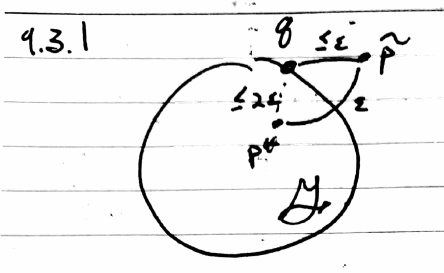
\includegraphics[width=0.7\textwidth]{figures/9-3-1.png}
        \caption{Given $D(p^*, \tilde{p}) \leq \eps$, $p^* \in \cG$, and
            $q$ is the projection of $\tilde{p}$ onto $\cG$ under $D$, we must
            have $D(\tilde{p}, q) \leq \eps$ and by triangle inequality
            $D(p^*, q) \leq 2\eps$
        }
    \end{figure}

    So $D(p^*, q) \leq 2 \eps$ and we can conclude
    \begin{align}
        \fm \geq L(p^*, \theta^*(q))
    \end{align}
\end{proof}

For now, we will specialize to the case $D = \TV$ and $L(p,  \theta) = \|\theta - \mu(p^*)\|_2$.
Consider a Gaussian distributional assumption $\cG_{gauss} = \{\cN(\mu, I) : \mu \in \RR^{d}\}$.

\begin{lemma}\label{lem:gauss-tv}
    $\TV(\cN(\mu, I), \cN(\mu', I)) \asymp \Theta(\min(\|\mu - \mu'\|_2, 1))$

    Therefore
    \begin{align}
         \fm(\cG_{gauss}, \eps) = \sup_{\substack{p,q \in \cG\\ \TV(p,q) \leq 2 \eps}} \|\mu(p) - \mu(q)\|_2 = \Theta(\eps)
    \end{align}
    for sufficiently small $\eps$.
\end{lemma}

\begin{proof}
    We first prove the 1D case. By translational symmetry, we can translate both
    distributions while preserving $\|\mu - \mu'\|_2 \eqqcolon u$ so that wlog we may
    assume the two distributions are $p = \cN(\frac{u}{2}, 1)$ and $q = \cN(-\frac{u}{2}, 1)$.
    Then
    \begin{align}
        \TV(p,q)
        &= \frac{1}{2} \frac{1}{\sqrt{2\pi}} \int_{-\infty}^\infty \lvert e^{(t + u/2)^2/2} - e^{(t-u/2)^2/2}\rvert dt \\
        &= \frac{1}{\sqrt{2\pi}} \int_{-u/2}^{u/2} e^{-t^2/2} dt \label{eq:9-3-int}
    \end{align}
    where the last equality follows by cancelling the probability mass in the following picture:
    \begin{figure}[H]
        \centering
        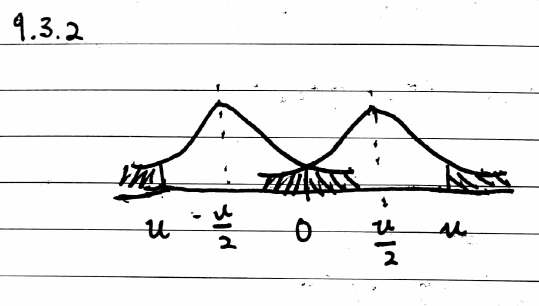
\includegraphics[width=0.7\textwidth]{figures/9-3-2.png}
        \caption{Both Gaussians exhibit identical $\pm \frac{u}{2}$ tails with opposite signs
            in the expression for $\TV$, so the $\TV$ is equivalent to the area in $[-u/2, u/2]$ drawn
            out by the pointwise max between the two PDFs. By symmetry, this is just twice the area
            inside $[-u/2, u/2]$ which after cutting and pasting integration areas (and cancelling the $1/2$
            in definition of $\TV$) is equal
            to the probability mass between $[-u/2,u/2]$ for a Gaussian.}
    \end{figure}

    Note that $e^{-t^2/2} \geq \frac{1}{2}$ if $\lvert t \rvert < 1$, so $\TV = \Omega(\min(u,1))$
    which can be seen by splitting the integral and examining the two cases where
    $\frac{u}{2} > 1$ (which yields the $1$) and $\frac{u}{2} < 1$ (which yields the $u$).

    Similarly, $e^{-t^2/2} \leq 1$ for all $t > 0$ so $\TV = O(\min(u,1))$.

    To generalize to higher dimensions, note identity covariance implies rotational invariance so we can
    rotate and translate such that the two means are on the first coordinate axis and separated
    by $\|\mu - \mu'\| = \lvert \mu_1 - \mu_1' \rvert$. In particular, $\mu_i = 0$ for $i \neq 1$ hence
    in the $\TV$ expression they can be factored out and integrated to $1$ to reduce to the 1D case.
\end{proof}

\subsection{Midpoint lemma and resilience}

As a less restrictive family, consider distributions with bounded covariance:
\begin{align}
    \cG_{cov}(\sigma)
    &= \{ p : \ex_p[(X - u)(X - u)'] \preceq \sigma^2 I\}
\end{align}

We begin with an important lemma which will be used to prove the modulus of continuity for $\cG_{cov}$
and generalized in the following section.
\begin{lemma}[Midpoint lemma]\label{lem:midpoint}
    If $\TV(p,q) \leq \eps$ then exists a \emph{midpoint} distribution $r$ such that
    $r \leq \min\{\frac{p}{1 - \eps}, \frac{q}{1 - \eps}\}$ and
    \begin{enumerate}
        \item $r(x) \leq \frac{p(x)}{1 - \eps}$ for all $x$
        \item $r$ is an \emph{$\epsilon$-deletion of $p$} (obtained by deleting $\epsilon$ mass from $p$)
        \item $r = p \vert_{E}$ for $p(E) \geq 1 - \eps$ where $E \mid X$ has probability $1$ if $p(x) \leq q(x)$ and $\frac{q(x)}{p(x)}$ if $p(x) > q(x)$
    \end{enumerate}
\end{lemma}

\begin{proof}
    The midpoint distribution is given by $r = \frac{\min(p,q)}{1 - \TV(p,q)}$ and is obtained from $p$
    by deleting probability mass from $q$ and renormalizing.
    \begin{figure}[H]
        \centering
        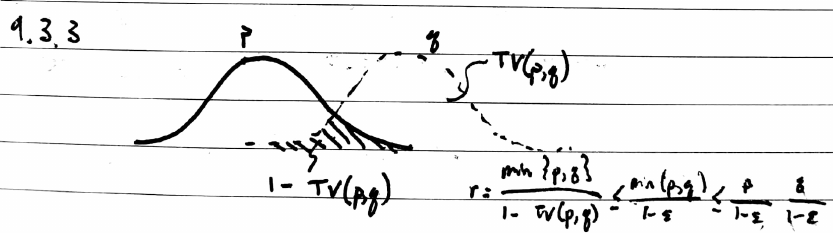
\includegraphics[width=0.6\textwidth]{figures/9-3-3.png}
        \caption{The midpoint distribution $r = \frac{\min(p,q)}{1 - \TV(p,q)}$ can be reached
        from both $p$ and $q$ by deleting $\epsilon$-mass and renormalizing.}
    \end{figure}
    Specifically, we delete
    $q(x) - p(x)$ mass from all points in $\{ x : q(x) > p(x) \}$, the integral of which is precisely
    equal to the total variation distance. This means that we must renormalize by $1 - \eps$ to ensure
    $r$ is a proper distribution.
\end{proof}

\begin{corollary}\label{corr:mod-cont-cov}
    $\fm(\cG_{cov}(\sigma), \eps) = O(\sigma \sqrt{\eps})$
\end{corollary}

\begin{proof}
    Take $p, q \in \cG_{cov}$ such that $\TV(p, q) \leq \eps$.
    By \cref{lem:midpoint}, there exists a midpoint distribution
    $r = p \mid_E$ for which
    \begin{align}
        \ex_r[X - \mu(p)]
        &= \ex_p[X - \mu(p) \mid \underbrace{E}_{1 - \eps}]
        = \frac{-\eps}{1 - \eps} \ex_p[X - \mu(p) \mid \underbrace{E^c}_{\eps}]
    \end{align}
    where the last equality follows from
    \begin{align}
        0
        &= \ex_p[X - \mu(p)]
        = \underbrace{p(E)}_{1-\epsilon} \ex_p[ X - \mu \mid E] + \underbrace{p(E^c)}_{\epsilon} \ex_p[X - \mu \mid E^c]
    \end{align}
    (This is a common trick for moving from conditioning on an event to
    conditioning on its complement in zero mean functionals).

    (Chebyshev in $\RR^d$) By linearity of expectation and Jensen's inequality
    \begin{align}
        \| \ex_p[X - \mu(p) \mid E^c] \|_2
        &= \sup_{\|v \|_2 \leq 1} \braket{\ex_p[X - \mu(p) \mid E^c], v} \\
        &= \sup_{\|v\|_2 \leq 1} \ex_p [\braket{X - \mu(p), v} \mid E^c] \\
        &\leq \sup_{\|v \|_2 \leq 1} \sqrt{\ex_p[\braket{X - \mu(p), v}^2 \mid E^c]}
    \end{align}
    Note $\ex_p[\braket{X - \mu(p), v}^2]
    = \Var_p[\braket{X - \mu(p), v}]
    = v^\top \Cov_p(X) v \leq \sigma^2$ so
    \begin{align}
        \| \ex_p[X - \mu(p) \mid E^c] \|_2
        &\leq \sqrt{\frac{\sigma^2}{\Pr[E^c]}}
        = \frac{\sigma}{\sqrt{\eps}}
        \label{eq:9-3-cheb-cov-control}
    \end{align}
    As a result, we have
    \begin{align}
        \|\mu(r) - \mu(p)\|_2 = \|\ex_r[X - \mu(p)]\|_2 \leq \frac{\eps}{1 - \eps} \frac{\sigma}{\sqrt{\eps}} \leq 2 \sigma \sqrt{\eps}
    \end{align}
    for $\eps < 1/2$.
    A similar argument involving $q$ gives $\|\mu(r) - \mu(q)\|_2 \leq 2 \sigma \sqrt{\eps}$
    so by triangle inequality $\|\mu(p) - \mu(q)\|_2 \leq 4 \sigma \sqrt{\eps}$.
\end{proof}

\begin{remark}
    Unlike the trimmed mean, there is no dependence on $d$ here.
    This means that the MDF remains a good robust estimator even in high dimensions!
\end{remark}

The above proof utilizes two key ingredients:
\begin{itemize}
    \item The midpoint property of $\TV$; both $p$ and $q$ are close to some $\eps$-deletion $r$
    \item The bounded tails (second moment) of $\cG_{cov}$, which is used to control how close $\mu(r)$
    and $\mu(p)$ are in \cref{eq:9-3-cheb-cov-control}
\end{itemize}

The previous proof can be suitably generalized to yield a modulus of continuity bound
for other families:
\begin{definition}[Resilient distribution]\label{def:resilience}
    A distribution is $(\rho, \eps)$-resilient if
    \begin{align}\label{eq:resilience-property}
        r \leq \frac{p}{1 - \eps} \implies \|\ex_r[X] - \ex_p[X]\|_2 \leq \rho
    \end{align}
    In other words, for any (not just midpoint) $\eps$-deletion $r$ the mean does not change in
    norm by more than $\rho$. Equivalently (e.g. when $p$ does not have a density) we can view $r = p \mid_E$
    for an event $E$ and use the definition
    \begin{align}
        p(E) \geq 1 - \eps \implies \|\ex_p[X \mid E] - \ex_p[X]\| \leq \rho
    \end{align}

    We let $\cG_{TV}(\rho, \epsilon)$ be the set of all $(\rho, \epsilon)$-resilient distributions.
\end{definition}

\begin{remark}
    This definition is only applicable for mean estimation under squared error loss.
\end{remark}

\begin{figure}[H]
    \centering
    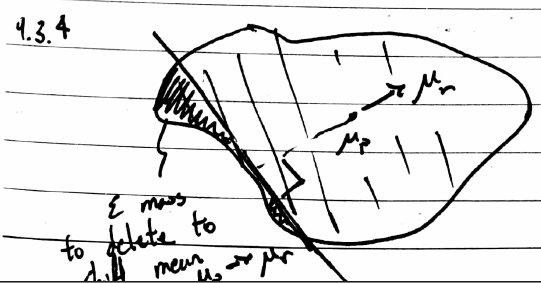
\includegraphics[width=0.5\textwidth]{figures/9-3-4.png}
    \caption{Deleting $\eps$ mass from a resilient distribution $p$ shifts the mean by a controlled
    amount $\|\mu_p - \mu_r\|_2 \leq \rho$.}
\end{figure}

\begin{example}\label{eg:bdd-cov-resilient}
    \cref{corr:mod-cont-cov} shows $\cG_{cov}(\sigma) \subset \cG_{TV}(2 \sigma \sqrt{\eps}, \eps)$
\end{example}

\begin{example}
    \cref{lem:gauss-tv} shows $\cG_{gauss}(\sigma) \subset \cG_{TV}(\eps \sqrt{\log \frac{1}{\eps}}, \eps)$
\end{example}

Combining with \cref{prop:mdf-modulus-error-bound}, for squared error loss we can say
\begin{corollary}[Modulus of continuity bound for resilient distributions]\label{corr:mod-bound-resilient}
    \begin{align}
        \fm(\cG_{TV}(\rho, \eps), \eps) \leq 2 \rho
    \end{align}
\end{corollary}
\begin{proof}
    For any $p,q \in \cG_{\TV}$,
    use \cref{lem:midpoint} to get a midpoint distribution
    and then \cref{eq:resilience-property} with triangle inequality to control the squared error loss.
\end{proof}
So we can always project onto the family of resilient distributions to get a MDF
estimator which has loss independent of $d$.

\subsection{Orlicz norms}

\begin{definition}[Orlitz function / norm]
    An \emph{Orlicz function} $\psi : \RR_{\geq 0} \to \RR_{\geq 0}$ is
    \begin{enumerate}
        \item Convex
        \item Non-decreasing
        \item $\psi(0) = 0$, $\psi(x) \to \infty$ as $x \to \infty$
    \end{enumerate}

    Given an Orlicz function $\psi$, the \emph{Orlicz norm} or $\psi$-norm of a
    random variable $X$ is
    \begin{align}
        \|X\|_\psi &= \inf \left\{t : \ex \psi\left(\frac{\lvert X \rvert}{t} \right) \leq 1 \right\}
    \end{align}
    For multivariate $X \in \RR^d$, define
    \begin{align}
        \|X\|_\psi = \inf \left\{t > 0 : \sup_{v \in \cS^{d-1}} \|\braket{X, v}\|_\psi \leq t \right\}
        \label{def:orlicz-norm-multivar}
    \end{align}
    In other words, $X$ has bounded $\psi$-norm if all of its one dimensional projections do.

    Let $\cG_\psi(\sigma) = \{ X : \|X - \ex[X]\|_\psi \leq \sigma \}$.
\end{definition}

\begin{example}
    $\psi(x) = x^k$ gives $\|X\|_\psi = \left(\ex[\lvert X \rvert^k]\right)^{1/k}$,
    which looks like $L_p$ norms. In fact, these are precisely distributions with bounded $k$th moments.

    For $\psi(x) = x^2$, we have $\cG_{\psi}(\sigma) = \cG_{cov}(\sigma)$.
\end{example}

\begin{definition}[Sub-Gaussian/Sub-Exponential]\label{def:sub-gaussian-sub-exp-orlicz}
    For $\psi_2(x) = e^{x^2} - 1$, $\cG_{\psi_2}(\sigma)$ are called the $\sigma$-sub-Gaussian random variables.

    For $\psi_1(x) = e^x - 1$, $\cG_{\psi_1}(\sigma)$ are called the $\sigma$-sub-exponential random variables.
\end{definition}

The next proposition shows that any distribution with bounded Orlicz norm is resilient.
\begin{proposition}[Bounded Orlicz norm implies resilience]\label{lem:orlicz-norm-resilient}
    $\cG_{\psi}(\sigma) \subset \cG_{TV}(2 \sigma \eps \psi^{-1}(\frac{1}{\eps}), \eps)$
    if $\eps < 1/2$.

    $\psi(x) \to \psi^{-1}(x) = \sqrt{x} \to \eps \psi^{-1}(1/\eps) = \sqrt{\eps}$
\end{proposition}

\begin{proof}
    \begin{align}
        \|\ex_r[X] - \ex_p[X]\|_2
        &= \|\ex_p[X - \mu \mid \underbrace{E}_{p(E) = 1 - \eps} ]\|_2
        = \frac{\eps}{1 - \eps} \| \ex_p [ X- \mu \mid E^c] \|
    \end{align}
    Focusing in on the expectation term
    \begin{align}
        \| \ex_p[X - \mu \mid E^c] \|_2
        &= \sup_{\|v\|_2 = 1} \ex_p[\braket{X - \mu, v} \mid E^c]
    \end{align}
    By Jensen's inequality, convexity of $\psi$ (equivalently concavity of $\psi^{-1}$),
    definition of multivariate Orlicz norm (\cref{def:orlicz-norm-multivar}),
    and monotonicity of $\psi$, we have
    \begin{align}
        \| \ex_p[X - \mu \mid E^c] \|_2
        &= \sup_{\|v\|_2 = 1} \sigma \left(
            \ex_p\left[(\sigma \psi^{-1} \circ \psi)\left( \frac{\lvert \braket{X - \mu, v} \rvert}{\sigma} \right) \mid E^c\right]
        \right) \\
        &\leq \sup_{\|v\|_2 = 1} \sigma \psi^{-1}\left(
            \ex_p\left[\psi\left( \frac{\lvert \braket{X - \mu, v} \rvert}{\sigma} \right) \mid E^c\right]
        \right) \\
        &\leq \sup_{\|v\|_2 = 1} \sigma \psi^{-1}\left(
            \underbrace{\ex_p\left[\psi\left( \frac{\lvert \braket{X - \mu, v} \rvert}{\sigma} \right) \right]}_{\leq 1}
            \underbrace{\frac{1}{\Pr[E^c]}}_{\frac{1}{\eps}}
        \right) \\
        &\leq \sigma \psi^{-1}(\frac{1}{\eps})
    \end{align}
\end{proof}

\section{9/5/2019}

\subsection{Recap}

\begin{itemize}
    \item Minimum distiance functionals: good error, bounded by modulus of continuity $\fm$
    \item Resilience $\implies$ bounded $\fm$
    \item Bounded Orlicz $\psi$-norm $\implies$ resilience
\end{itemize}
This lecture:
\begin{itemize}
    \item Want to analyze $X_1, \ldots, X_n$
    \item ``The empirical average converges to the mean if $n$ is large''
    \item Two steps:
    \begin{enumerate}
        \item Show \emph{concentration inequality}: bound variation of $p$ in terms of $\sigma$
        \item Show \emph{composition property}: $\sigma$ gets smaller as we take more independent samples
    \end{enumerate}
\end{itemize}

\subsection{Concentration Inequalities and Composition}

\begin{example}
    A slot machine has expected payout of \$5 and always pays out positive.
    
    \textbf{Question}: What is the maximum probability of $\geq \$100$?
    
    \textbf{Answer}: 5\%, by letting $P(X=\$0) = 0.95$ and letting $P(X=\$100) = 5\%$.
\end{example}

The preceding example is an instance of \nameref{thm:markov}:
\begin{theorem}[Markov's Inequality]\label{thm:markov}
    If $X \geq 0$ has bounded first moment, then
    \begin{align}
        \Pr[X \geq t \ex[X]] &\leq \frac{1}{t}
    \end{align}
\end{theorem}
\begin{proof}
    \begin{align}  
        t \ex[X] \ind\{X \geq t \ex[X]\} &\leq X
    \end{align}
    Take expectation of both sides and rearrange.
\end{proof}

\nameref{thm:markov} has a nice composition property:
\begin{theorem}[Composition of Markov for sums]\label{thm:markov-composition}
    Let $X_1, X_2 \sim p$ with mean $\mu$.
    \begin{align}
        \Pr\left[ \frac{X_1 + X_2}{2} \geq t \mu \right] &\leq \frac{1}{t}
    \end{align}
\end{theorem}
This is because $\ex[(X_1 + X_2) / 2] = \mu = \ex[X_1] = \ex[X_2]$.

We can apply \nameref{thm:markov} to $Z = f(X)$ for $f : \RR \to \RR_{\geq 0}$
and get a family of inequalities
(provided $\ex[f(X)] < \infty$).
For example, taking $Z = (X - \mu)^2$ and assuming $\ex[Z] = \Var[X] = \sigma^2 < \infty$ yields
\begin{theorem}[Chebyshev's inequality]\label{thm:chebyshev}
    \begin{align}
        \Pr[\lvert X - \mu\rvert \geq t \sigma] \leq \frac{1}{t^2}
    \end{align}
\end{theorem}

Analogous to \myref{thm:markov-composition},
a composition property for \nameref{thm:chebyshev} would require a composition property involving variances:
\begin{theorem}[Variances add for independent RVs]
    If $\{X_i\}_{i=1}^n$ are independent, then
    \begin{align}
        \Var\left[ \sum_{i=1}^n X_i \right] = \sum_{i=1}^n \Var[X_i]
    \end{align}
\end{theorem}

\begin{example}[Concentration of empirical average]
    Let $X_1, \ldots, X_n \simiid p$ with mean $\mu$ and variance $\sigma^2$.
    Let $S = \sum_i^n X_i$ and $\frac{S}{n}$ the empirical average. Then
    \begin{align}
        \Var[S/n] = n \Var[X/n] = n \frac{\sigma^2}{n^2} = \frac{\sigma^2}{n}
    \end{align}
    Hence, the standard deviation of the empirical average $\frac{S}{n}$ is $\sigma_{avg} = \frac{\sigma}{\sqrt{n}}$.
    \nameref{thm:chebyshev} then yields
    \begin{corollary}\label{cor:chebyshev-empirical-avg-concentration}
        \begin{align}
            \Pr\left[
                \left\lvert \frac{S}{n} - \mu \right\rvert \geq t \frac{\sigma}{\sqrt{n}}
            \right] &\leq \frac{1}{t^2}
        \end{align}
    \end{corollary}
\end{example}

The $t^{-2}$ quadratic decay in \cref{cor:chebyshev-empirical-avg-concentration} is tight, as the following
proposition shows:
\begin{proposition}[Lower bounds for Chebyshev]
    There exists $X_1, \ldots, X_n$ pairwise independent, bounded in $[-1, 1]$, mean zero, variance one, such that
    \begin{align}
        \Pr\left[\sum_{i=1}^n X_i = n \right] = \frac{1}{n}
    \end{align}
    Consequently, \cref{cor:chebyshev-empirical-avg-concentration} (with $\mu=0$, $\sigma=1$, and $t = \sqrt{n}$)
    is tight.
\end{proposition}
\begin{proof}
    Flip $k$ independent coins and let $n = 2^k$. For any subset $\emptyset \subsetneq S \subset [k]$, define the random variable
    \begin{align}
        X_S = \begin{cases}
            1 &\text{\# heads in $S$ is even} \\
            -1 &\text{\# heads in $S$ is odd}
        \end{cases}
    \end{align}
    $X_S$ is mean zero, variance one, bounded $[-1,1]$, and pairwise
    independent (since the coin flips are). The event $\{ \sum_{i=1}^n X_i = n \}$
    occurs iff all of the coins land tails, which occurs with probability $2^{-k} = \frac{1}{n}$.
\end{proof}

\subsection{Failure of composition of higher moments and Rosenthal's inequality}\label{ssec:rosenthals-inequality}

To try to extend \nameref{thm:chebyshev}, we can consider applying \nameref{thm:markov} to
$Z = f(X) = (X - \mu)^4$ to get:
\begin{theorem}
    \begin{align}
        \Pr[\lvert X - \mu\rvert \geq t \ex[Z]^{1/4} ] &\leq \frac{1}{t^4}
    \end{align}
\end{theorem}
However, the composition property fails here since
for $\ex[X_1] = \ex[X_2] = 0$ we find
\begin{align}
    \ex[(X_1 + X_2)^4]
    &= \ex[X_1^4] + \ex[X_2^4]
    + 4 \cancelto{0}{\ex[X_1]} \ex[X_2^3]
    + 4 \cancelto{0}{\ex[X_2]} \ex[X_1^3]
    + \underbrace{6 \ex[X_1^2 X_2^2]}_{\geq 0}\label{eq:9-5-4th-moment-nonadditive}
\end{align}
Thus, the fourth moment of a sum can be larger than the sum of the fourth moments.

In general, higher moments don't add.
One method to work around this is to work with cumulants (see \cref{ssec:cumulants-additive}).
An alternative method is through Rosenthal's inequality:

\begin{lemma}[Rosenthal's inequality]\label{lem:rosenthal-ineq}
    If $X_1,\ldots, X_n$ are independent mean zero random variables with finite $p$th moments, then
    \begin{align}
        \ex\left[\left\lvert \sum_{i=1}^n X_i \right\rvert^p\right]
        &\leq O(p)^p \sum_{i=1}^n \ex[\lvert X_i \rvert^p]
        + O(\sqrt{p})^p \left( \sum_{i=1}^n \ex[X_i^2] \right)^{p/2}
    \end{align}
\end{lemma}

How can we use \nameref{lem:rosenthal-ineq}?
Suppose $X_1, \ldots, X_n \simiid \pi$ with $\ex[\lvert X \rvert^p] = k^p$
and $\ex[X^2] = \sigma^2$. Let $S = \sum_{i=1}^n X_i$.
Then
\begin{align}
    \ex[\lvert S \rvert^p ] &\leq O(p)^p n k^p + O(\sqrt{p})^p (n \sigma^2)^{p/2} \\
    \ex[\lvert S \rvert^p]^{1/p} &\leq O(p k n^{1/p} + \sqrt{p} \sigma n^{1/2}) \\
    \ex\left[ \left\lvert \frac{S}{n} \right\rvert^p \right]^{1/p}
    &\leq O(p k n^{-(1-\frac{1}{p})} + \sqrt{p} \sigma n^{-1/2})
\end{align}
Hence, all of the $p$th moments of the empirical mean $\frac{S}{n}$ decay in $n$,
so the empirical mean concentrates about the population mean as the number of samples $n \to \infty$.

\subsection{Exponential tails and Chernoff bounds}

Another approach which can yield exponential tail bounds is through the \nameref{def:moment-generating-function}. 
\begin{definition}[Moment Generating Function]\label{def:moment-generating-function}
    Let $X$ be a random variable with bounded moments.
    The \emph{moment generating function} (MGF) of $X$ is
    \begin{align}
        m_X(\lambda)
        &= \ex \exp(\lambda (X - \mu))
        = 1 + \lambda \ex[x] + \frac{\lambda^2}{2} \ex[X^2]  \frac{\lambda^3}{6} \ex[X^3] + \cdots
    \end{align}
\end{definition}

MGFs satisfy a desirable composition property enabling us to easily compute the MGF of a sum in terms
of the MGFs of the summands:
\begin{lemma}[Composition property for MGFs]\label{lem:mgf-sum-composition}
    If $X_1, \ldots, X_n$ are independent, then
    \begin{align}
        m_{\sum_i^n X_i}(\lambda) = \prod_i^n m_{X_i}(\lambda)
    \end{align}
\end{lemma}
\begin{proof}
    Exponential of sum is product of exponentials, independence of $X_i$ allows splitting
    of $\ex$.
\end{proof}

Another strong advantage of working with moment generating functions is that we can use them to
get exponentially decaying tail bounds:

\begin{theorem}[Chernoff's bound]\label{thm:chernoff}
    For $\lambda \geq 0$,
    \begin{align}
        \Pr[X - \mu \geq t] \leq \inf_{\lambda \geq 0} m_X(\lambda) e^{-\lambda t}
    \end{align}
\end{theorem}

\begin{proof}
    $X - \mu \geq t$ implies $\exp(\lambda(X - \mu)) \geq e^{\lambda t}$.
    The same technique used to prove \nameref{thm:chebyshev} (with $f(x) = e^{\lambda x}$) gives
    \begin{align}
        \Pr[\exp(\lambda (X - \mu)) \geq e^{\lambda t}]
        \leq e^{-\lambda t} m_X(\lambda)
    \end{align}
\end{proof}

\begin{example}[sub-exponential Chernoff bound]\label{eg:sub-exponential-chernoff}
    Recall from \myref{def:sub-gaussian-sub-exp-orlicz} that $\sigma$-sub-exponential means
    bounded Orlicz norm $\|X - \mu\|_\psi = \ex\left[\psi\left(\frac{\lvert X - \mu \rvert}{\sigma}\right)\right] \leq 1$
    for $\psi(x) = e^x - 1$. \nameref{thm:chernoff} then implies
    \begin{align}
        \ex[\exp(\lvert X - \mu \rvert / \sigma) - 1] &\leq 1\\
        \ex[\exp(\lvert X - \mu \rvert / \sigma)] &\leq 2\\
        m_X(1/\sigma)
        = \ex \exp\left(\frac{x - \mu}{\sigma}\right)
        \leq \ex \exp\left(\frac{\lvert x - \mu \rvert}{\sigma}\right)
        &\leq 2 \\
        \Pr[X - \mu \geq t] &\leq 2 \exp(-t / \sigma)
    \end{align}
    This explains the name ``sub-exponential'': the tail probabilities decay faster than an exponential.
\end{example}

\begin{example}[sub-Gaussian Chernoff bound]\label{eg:sub-gaussian-chernoff}
    Recall from \myref{def:sub-gaussian-sub-exp-orlicz} that $\sigma$-sub-Gaussian means
    bounded Orlicz norm $\|X - \mu\|_\psi$ with $\psi(x) = e^{x^2} - 1$.
    Hence, $\ex[\exp((X - \mu)^2 / \sigma^2)] \leq 2$ and
    \begin{align}
        m_X(\lambda)
        = \ex \exp(\lambda (X - \mu))
        &\leq \exp(\lambda^2 \sigma^2 / 4) \cancelto{2}{\ex \exp((X - \mu)^2 / \sigma^2)} ]
        = 2 \exp(\lambda^2 \sigma^2 / 4)
    \end{align}
    where we have used inequality $ab \leq \frac{a^2}{4} + b^2$ to conclude
    \begin{align}
        \lambda (X - \mu) &\leq \frac{\lambda^2 \sigma^2}{4} + \frac{(X - \mu)^2}{\sigma^2}
    \end{align}
    
    \begin{remark}
        We can also show
        \begin{align}
            m_X(\lambda)
            \leq \exp\left(\frac{1}{2} \lambda^2 (\sigma')^2\right)
        \end{align}
        where $\sigma' \leq \sqrt{3} \sigma$. This is sometimes taken as definition of $\sigma'$-sub-Gaussian.
    \end{remark}
    
    Applying \nameref{thm:chernoff} shows
    \begin{align}
        \Pr[X - \mu \geq t]
        &\leq \inf_{\lambda \geq 0} m_X(\lambda) e^{-\lambda t} \\
        &\leq \inf_{\lambda \geq 0} \exp\left( \frac{1}{2} \lambda^2 (\sigma')^2 - \lambda t \right) \\
        &= \exp\left( -\frac{t^2}{2 (\sigma')^2}\right)
    \end{align}
    This explains the name ``$\sigma'$-sub-Gaussian'': the tail probabilities are decaying faster than those of a Gaussian
    distribution with variance $\sigma'$.
    
    By \myref{lem:mgf-sum-composition}, we have that the sum $S = \sum_i^n X_i$ of $\sigma'$-sub-Gaussian RVs
    is itself $\frac{\sigma'}{\sqrt{n}}$-sub-Gaussian and
    satisfies the tail bound
    \begin{align}
        \Pr\left[\frac{S}{n} - \mu \geq t\right]
        &\leq \exp\left( - \frac{n t^2}{2 (\sigma')^2} \right)
        = \exp\left( - \frac{n t^2}{6 \sigma^2} \right) \label{eq:sum-sub-gaussian-tail-bound}
    \end{align}
    This yields our desired exponential rate of concentration.
\end{example}

\subsection{Bounded random variables}

Bounded RVs are sub-Gaussian, but we can get tighter bounds than the previous example.
Let $X - \mu \in [-M, M]$. Then
\begin{align}
    \ex \exp \frac{\lvert X - \mu \rvert}{M^2 / \log 2} \leq \ex \exp \log 2 = 2
\end{align}
Hence $X$ is sub-Gaussian with parameter $\sigma = \sqrt{\frac{M^2}{\log 2}}$
and we can use \cref{eq:typical-sup-via-concentration} to get tail bounds.
More generally:
\begin{corollary}[Hoeffding's inequality]\label{corr:hoeffding-inequality}
    Let $X_1,\ldots, X_n \in [a,b]$ be bounded independent mean zero random variables. Then
    \begin{align}
        \Pr\left[\frac{S}{n} - \mu \geq t \right] &\leq \exp\left( - \frac{2 n t^2}{(a - b)^2} \right)
    \end{align}
\end{corollary}

\begin{proof}
    Bound MGF (tighter than what we are doing here) and apply \nameref{thm:chernoff}.
\end{proof}

\nameref{corr:hoeffding-inequality} shows that an empirical average of independent bounded random variables
converges to its mean at a rate of $\frac{1}{\sqrt{n}}$ with tails that decay at least as fast as Gaussians.
Compare this against the $\frac{1}{n}$ rate for sub-exponentials we found in \cref{eg:sub-exponential-chernoff}
and the quadratic $\frac{1}{t^2}$ tails from \nameref{thm:chebyshev} (which only required finite second moments).

\subsection{Aside: Cumulants are additive}\label{ssec:cumulants-additive}

We saw in \cref{ssec:rosenthals-inequality} that fourth moments are additive.
While \myref{lem:mgf-sum-composition} provides a convenient composition property for moment generating functions,
the existence of MGFs requires all moments of the random variable to be bounded. In particular, this excludes
random variables with fat tails.

To construct additive quantities, we can start with MGF (multiplicative)
and take log (which is additive)
\begin{align}
    K_X(\lambda)
    &= \log \ex \exp(\lambda (X - \mu)) \\
    &= \log\left(
        1 + \ex[(X - \mu)^2] \frac{\lambda^2}{2} + \ex[(X - \mu)^3] \frac{\lambda^3}{6} + \cdots
    \right) \label{eq:cumulant-function-taylor-series} \\
    &= 1 + \sum_{n=1}^\infty \frac{\kappa_n(X)}{n!}\lambda^n 
\end{align}
This leads to the cumulant generating function:
\begin{definition}[Cumulants]
    The \emph{cumulant generating function} for a random variable $X$ is
    \begin{align}
        K_X(\lambda) &= \log \ex \exp(\lambda X) = 1 + \sum_{n=1}^\infty \frac{\kappa_n(X)}{n!}\lambda^n 
    \end{align}
    $\kappa_n(X)$ is called the $n$th cumulant of $X$.
\end{definition}
Notice $K_{X + Y}(\lambda) = K_X(\lambda) + K_Y(\lambda)$ so we have additivity of the CGF and consequentially
\begin{align}
    \kappa_4(X + Y) = \kappa_4(X) + \kappa_4(Y)
\end{align}
Contrast this to \cref{eq:9-5-4th-moment-nonadditive}.

However, computing the cumulants require Taylor expanding $\log$ using the infinite
series in \cref{eq:cumulant-function-taylor-series} as the argument and are laborious to work with.
To handle heavy tails, it may be easier to use \nameref{lem:rosenthal-ineq} instead.

\subsection{Max of n sub-Gaussians}

Let $X_1, \ldots, X_n \sim p$, $p$ is $\sigma$-sub-Gaussian. A simple union bound shows:
\begin{theorem}[Max of sub-gaussian bound]\label{thm:max-sub-gaussian}
    \begin{align}
        \Pr[X_1 \lor \cdots \lor X_n \geq t]
        &\leq \sum_{i=1}^n \Pr[X_i \geq t]
        \leq n e^{-\frac{t^2}{2 \sigma^2}}
    \end{align}
    So in particular if $t \gg \sigma \sqrt{\log n}$, then its not likely the max will exceed $t$.
\end{theorem}
\section{9/10/2019}

\subsection{Bounding suprema via concentration}

The typical type of quantity we will focus on here is
\begin{align}
    \underbrace{\sup_{v \in V}}_{\text{bound by discretization}}
    \underbrace{\frac{1}{n} \sum_{i=1}^n \left(X_i(v) - \ex[X(v)] \right)}_{\text{bound for fixed $v$ via concentration}}\label{eq:typical-sup-via-concentration}
\end{align}
When $V$ is finite, a simple union bound can be applied.
To deal with infinitely large $\lvert V \rvert$, we will need to first discretize $V$ into
a finite set.

\subsection{Warmup: max of sub-Gaussian}

Suppose $\{X_i\}_{i=1}^n \simiid p$ where $p$ is mean zero and $\sigma$-sub-Gaussian.
How big is $\max_{i=1}^n X_i$?

\begin{lemma}\label{lem:concentration-max-sub-gaussian}
    With probability $\geq 1 - \delta$
    \begin{align}
        \max_{i=1}^n X_i \in O\left(\sigma \sqrt{\log n + \log \frac{1}{\delta}} \right)
    \end{align}
\end{lemma}

\begin{proof}
    By union bound, iid, and \nameref{eg:sub-gaussian-chernoff}
    \begin{align}
        \Pr\left[\max_{i=1}^n X_i \geq t \right] 
        &\leq n \Pr[X_1 \geq t]
        \leq n \exp\left(-\frac{t^2}{2 \sigma^2}\right)
    \end{align}
    To ensure this failure event occurs with probability $\leq \delta$, we need
    \begin{align}
        n \exp\left(-\frac{t^2}{2 \sigma^2}\right) &\leq \delta \\
        \frac{t^2}{2 \sigma^2} &= \log n + \log \frac{1}{\delta} \\
        t &\leq \sigma \sqrt{2\left(\log n + \log \frac{1}{\delta} \right)}
    \end{align}
\end{proof}

If instead we were interested in $\max_{i=1}^n \lvert X_i \rvert$, then a union bound on the two
tail events $\{X_i \geq t\}$ and $\{-X_i \geq t\}$ (note $-X_i$ is still sub-Gaussian) gives
\begin{align}
    \Pr\left[\max_{i=1}^n \lvert X_i \rvert \geq t\right] &\leq 2 n \exp\left( -\frac{t^2}{2 \sigma^2} \right) 
    \label{eq:tail-bound-abs-value-two-factor}\\
    \max_{i=1}^n \lvert X_i \rvert &\in O\left( \sigma \left(\sqrt{\log 2 + \log n + \log \frac{1}{\delta}}\right) \right)
\end{align}

In later the next section, we will see how we can ``reduce'' an infinitely large $V$
into an exponentially large $N$ after which
we will use the same technique to bound the event $\{ \max_{i \in N} X_i \geq t \}$.
To get concentration, we will need the exponential tail bound to dominate the now exponentially large $n = \lvert N \rvert$
arising from the union bound over $N$.

\subsection{Maximum eigenvalue of random matrix}

Suppose $\{X_i \in \RR^d \}_{i=1}^n \simiid p$ with $p$ zero mean and $\sigma$-sub-Gaussian.

Recall from \myref{def:orlicz-norm-multivar} and \myref{def:sub-gaussian-sub-exp-orlicz}
that $X \in \RR^d$ is $\sigma$-sub-Gaussian if all its one dimensional projections are, that is:
\begin{align}
    \|X\|_\psi + 1
    &= \sup_{v \in \cS^{d-1}} \|\braket{v,X}\|_\psi + 1
    = \sup_{v \in \cS^{d-1}} \ex \exp\left(\frac{\braket{v, X}^2}{\sigma^2} \right)
    \leq 2\label{eq:9-10-recap-multivar-sub-gaussian}
\end{align}

We are interested in the (random) empirical covariance matrix
\begin{align}
    M = \frac{1}{n} \sum_{i=1}^n X_i X_i^\top
\end{align}
Specifically, we would like to understand how big $\|M\| = \lambda_{\max}(M)$ is.

\begin{proposition}\label{prop:9-10-cov-operator-norm}
    With probability $\geq 1 - \delta$
    \begin{align}
        \|M\| = O\left(\sigma^2 \left( 1 + \frac{d}{n} + \frac{\log \frac{1}{\delta}}{n} \right) \right)
    \end{align}
\end{proposition}

\begin{remark}
    \Cref{prop:9-10-cov-operator-norm} shows that:
    \begin{itemize}
        \item As $n \to \infty$, $\|M\| = O(\sigma^2)$ and does not depend on $d$.
        \item The population covariance operator norm $\|\ex X_i X_i^\top\| = O\left( \frac{\sigma^2}{n} \log \frac{1}{\delta} \right)$ is attained if $d = \Theta(n)$ (i.e. if the dimension grows at the same rate as $n$)
    \end{itemize}
\end{remark}


To relate back to the two-step strategy outlined in \cref{eq:typical-sup-via-concentration}, note
\begin{align}
    \|M\| &= \sup_{v \in \cS^{d-1}} v^\top M v
    = \sup_{v \in \cS^{d-1}} \frac{1}{n} \sum_{i=1}^n \braket{X_i, v}^2
\end{align}
This quantity looks promising as it is the sum of independent sub-Gaussian RVs.

Since $\braket{X_i, v}$ is $\sigma$-sub-Gaussian, $\braket{X_i, v}^2$ is $\sigma^2$-sub-exponential (\cref{def:sub-gaussian-sub-exp-orlicz}, or equivalently \cref{eq:9-10-recap-multivar-sub-gaussian})
and for any fixed $v \in \cS^{n-1}$ 
\begin{align}
    \ex \exp\left(\frac{\braket{X_i, v}^2}{\sigma^2}\right) &\leq 2 \\
    \ex \exp\left(\frac{n}{\sigma^2} \frac{1}{n} \sum_{i=1}^n \braket{X_i, v}^2 \right)
    = \prod_{i=1}^n \ex \exp \left(\frac{\braket{X_i, v}^2}{\sigma^2}\right) 
    &\leq 2^n 
\end{align}
where we used \nameref{lem:mgf-sum-composition} for the equality in the second line.

By \cref{thm:chernoff}, for fixed $v \in \cS^{d-1}$
\begin{align}
    \Pr[v^\top M v \geq t] \leq 2^n \exp\left(\frac{-n t}{2 \sigma^2}\right) \label{eq:9-10-conc-sum}
\end{align}
So we have accomplished the first step (showing the individual terms inside the $\sup$ concentrate for fixed $v$).

For the second step, we will take a sufficiently small discretization of the unit ball $\{\|v\|\leq 1\}$:
\begin{lemma}\label{lem:9-10-unit-ball-packing}
    There exists a finite set $N \subset \RR^d$ with $\lvert N \rvert \leq 9^d$ and 
    \begin{align}
        \sup_{v \in \cS^{d-1}} v^\top M v &\leq 2 \sup_{v \in N} v^\top M v
    \end{align}
\end{lemma}

Applying \cref{lem:9-10-unit-ball-packing}, a union bound, \cref{eq:9-10-conc-sum},
and bounding the failure probability by $\delta$
shows that
\begin{align}
    \Pr[ \|M\| \geq t ]
    &= \Pr\left[ \sup_{v \in \cS^{d-1}} v^\top M v \geq t \right]
    \leq 9^d 2^n \exp\left(\frac{-nt}{2 \sigma^2}\right) = \delta \\
    \frac{n t}{2 \sigma^2} &= d \log 9 + n \log 2 + \log \frac{1}{\delta} \\
    t &= O\left(\sigma^2 \left( \frac{d}{n} + 1 + \frac{\log 1/\delta}{n} \right)\right)
\end{align}

\begin{proof}[Proof of \cref{lem:9-10-unit-ball-packing}]
    Let $N$ be a maximal packing of $\Ball_1(0)$ in $\RR^d$
    such that $\|u - v\|_2 \geq \frac{1}{4}$ for all $u \neq v \in N$.
    
    As shown in \cref{fig:9-10-1}, if we place a $1/8$-radius ball at all the
    points in $N$ then (1) all the balls are disjoint and (2) the union of all the balls is
    contained in $\Ball_{9/8}(0)$ Therefore, by the (converse of the) pidgeonhole principle,
    $\lvert N \rvert \leq \frac{\Vol(\Ball_{9/8}(0))}{\Vol(\Ball_{1/8}(0))} = 9^d$.
    
    \begin{figure}[H]
        \centering
        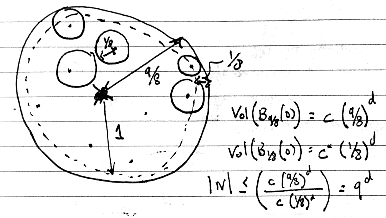
\includegraphics[width=0.6\textwidth]{figures/9-10-1.png}
        \caption{$1/8$-radius balls centered
            at all packing points are disjoint, the union of all these balls is contained in $B_{9/8}(0)$,
            so the cardinality $\lvert N \rvert \leq \left(\frac{9/8}{1/8}\right)^d = 9^d$.}
        \label{fig:9-10-1}
    \end{figure}
    
    Let $v \in \cS^{d-1}$ maximize $v^\top M v$
    and $u \in N$ such that $\|u - v\|_2 \leq \frac{1}{4}$.
    Such a $u$ must exist,
    otherwise $N \cup \{v\}$ is a larger $1/4$-packing which contradicts maximality of $N$.
    \begin{align}
        \|M\| - \lvert u^\top M u \rvert
        &= \lvert v^\top M v \rvert - \lvert u^\top M u \rvert \\
        &\leq \lvert v^\top M v - u^\top M u \rvert \\
        &= \lvert (u + v)^\top M (u - v) \rvert \\
        &\leq \underbrace{\|u + v\|_2}_{\leq 2} \|M\| \underbrace{\|u - v\|_2}_{\leq 1/4} \\
        &\leq \frac{1}{2} \|M\|
    \end{align}
    Hence $\|M\| \leq 2 u^\top M u \leq 2 \sup_{u \in N} u^\top M u$ as desired.
\end{proof}

\subsection{VC inequality and Symmetrization}

In this section, we will see how a family of events with certain geometric structure (which we will
quantify using VC-dimension) converges to its expectation at a rate dependent on the geometry.
In the process, we will encounter the technique of \emph{symmetrization}
(Prof. Steinhardt calls it ``bring your own randomness'') used to add additional randomness which
will be required to get concentration.

Let $\cH$ be a collection of functions $f : \cX \to \{0,1\}$ and $\{X_i \in \cX\}_{i=1}^n \simiid p$.
For $f \in \cH$, let
\begin{align}
    \nu(f) &= \ex_{x \sim p}[ f(x)] = \Pr_{x \sim p}[f(X) = 1] \\
    \nu_n(f) &= \frac{1}{n} \sum_{i=1}^n f(X_i) = \frac{1}{n} \#\{i : f(X_i) = 1\}
\end{align}
be the population and empirical averages respectively.

\textbf{Question}: How big is the discrepancy
\begin{align}
    D_n &= \sup_{f \in \cH} \lvert v_n(f) - v(f) \rvert
\end{align}

\textbf{Easy case}: $\lvert \cH \rvert < \infty$. Since $f(X_i)$ is bounded, apply \nameref{corr:hoeffding-inequality}
to the sum of independent bounded random variables to get:
\begin{align}
    D_n &= \max_{f \in \cH} \frac{1}{n} \sum_{i=1}^n (f(X_i) - \ex f(X)) \\
    \Pr\left[\frac{1}{n} \sum_{i=1}^n (f(X_i) - \ex f(X) \geq t \right] &\leq \exp(-2 n t^2)
\end{align}
A subsequent union bound over $\lvert \cH \rvert$ reveals
$t = O\left(\sqrt{\frac{1}{2n} \left( \log \lvert \cH \rvert + \log \frac{1}{\delta} \right)}\right)$

\textbf{More common case}: $\lvert \cH \rvert = \infty$. 
In this situation, we will bound $D_n$ using the geometry of $\cH$.
To do so, we will quantify the geometry using the following definitions:

\begin{definition}[Shattering number / VC dimension]
    The \emph{shattering number} of $\cH$ is
    \begin{align}
        V_{\cH}(\{x_i\}_{i=1}^n) &= \text{\# distinct} \{(f(x_1), \ldots, f(x_n)) : f \in \cH\} \\
        V_{\cH}(n) &= \max_{\lvert S \rvert = n} V_{\cH}(S)
    \end{align}
    It measures the number of possible ways to assign $\{0,1\}$ labels to $x_i$ which can be perfectly
    fit by $f \in \cH$.
    
    The \emph{VC dimension}
    \begin{align}
        vc(\cH) &= \max\{ n : V_{\cH}(n) = 2^n\}\label{eq:vc-dim-def}
    \end{align}
    It measures the largest cardinality $n$ such that for any set of points $S$ with cardinality $\lvert S \rvert = n$
    and any $\{0,1\}$ labelling of those points, some $f \in \cH$ can perfectly fit it.
\end{definition}

The shattering number is useful because instead of taking $\sup_{f \in \cH}$ of a term
involving $f$ only through $\{f(X_i)\}_{i=1}^n$, we can instead take the supremum over
$\{f(X_i)\}_{i=1}^n$ directly and only deal with $V_{\cH}(n)$ terms.

\begin{example}[VC dimension of half spaces]\label{eg:half-spaces-vc}
    Let $\cX = \RR^d$, $\cH = \text{half spaces} = \{f(x) = \ind[\braket{v,x} \geq \tau] : v \in \RR^d, \tau \in \RR \}$.
    Then $vc(\cH) = d+1$.
    
    We will see a proof next time, but for now consider an example where $d=2$.
    We can always separate 3 points by drawing a line, so $vc(\cH) \geq 3$.
    However, with 4 points there can be crossings (see \cref{fig:9-10-vc-hs}) which cannot be shattered.
        \begin{figure}[H]
        \centering
        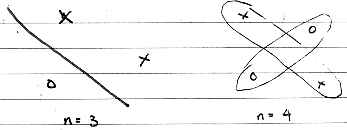
\includegraphics[width=0.6\textwidth]{figures/9-10-2.png}
        \label{fig:9-10-vc-hs}
        \caption{$n=3$ can always be shattered by a line, but the crossings possible when $n=4$ prevent this.}
    \end{figure}
\end{example}

Clearly by definition $V_\cH(n) = 2^n$ for all $n \leq vc(\cH)$.
When $n > vc(\cH)$, by \myref{eq:vc-dim-def} we have $V_\cH(n) < 2^n$.
The following lemma quantifies this and shows that the shattering number
is actually significantly smaller (growing polynomially in $n$ rather than exponentially):
\begin{lemma}[Sauer-Shelah]\label{lem:sauer-shelah}
    If $vc(\cH) = d$, then $V_{\cH}(n) \leq 2 n^d$.
\end{lemma}
While we will use this without proof, \nameref{lem:sauer-shelah} is the main reason why VC dimension
is useful for us: it allows us to convert the infinite supremum over $f \in \cH$ into a finite supremum over
$O(n^{\vc(\cH)})$ many terms of the form $\{f(X_i)\}_{i=1}^d$.

\begin{theorem}[VC inequality]\label{thm:vc-inequality}
    With probability $\geq 1 - \delta$
    \begin{align}
        D_n = O\left(\sqrt{\frac{vc(\cH) + \log \frac{1}{\delta}}{n}}\right)    
    \end{align}
\end{theorem}

\begin{proof}
    We will show something weaker, namely:
    \begin{align}
        \ex D_n &\leq O\left( \frac{vc(\cH) \log n}{n} \right)
    \end{align}
    The $\log \frac{1}{\delta}$ tail bound follows from McDarmid's inequality,
    and removing the extra $\log n$ refines the argument we will give using a tool called chaining.
    
    \textbf{Incorrect proof path}: Notice that
    \begin{align}
        D_n &= \sup_{f \in \cH} \left\lvert
            \underbrace{\frac{1}{n} \sum_{i=1}^n (f(X_i) - \ex f(X))}_{\Pr[\cdot \geq t] \leq \exp(-2 n t^2)}
        \right\rvert
    \end{align}
    So \nameref{corr:hoeffding-inequality} can be used to control the term inside the supremum.
    Let $vc(\cH) = d$.
    By \cref{lem:sauer-shelah}, there are only $O(n^d)$ distinct $(f(X_1), \ldots, f(X_n))$
    so a union bound implies $t = O\left(\sqrt{\frac{d \log n + \log \frac{1}{\delta}}{2n}}\right)$
    
    This is incorrect because applying Sauer-Shelah requires us to condition on a specific realization of $\{X_i\}_{i=1}^n$
    (after which we know there are at most $V_{\cH}(n)$ distinct values of $(f(X_1), \ldots, f(X_n))$).
    After conditioning, there's no randomness left for applying \nameref{corr:hoeffding-inequality} to get concentration.
    
    \textbf{Solution}: Introduce additional randomness using \emph{symmetrization}.
    Introduce independent copies $X_i'$ and note
    \begin{align}
        \ex[D_n] &= \ex_{X_1, \ldots, X_n}\left[\sup_{f \in \cH} \left\lvert
            \frac{1}{n} \sum_{i=1}^n f(X_i) - \ex f(X)
        \right\rvert \right] \\
        &= \ex_{X_1, \ldots, X_n} \left[ \sup_{f \in \cH} \left\lvert \ex_{X_1', \ldots, X_n'} \left[
            \frac{1}{n} \sum_{i=1}^n (f(X_i) - f(X_i'))
        \right]\right\rvert\right]
    \end{align}
    $\lvert \cdot \rvert$ is convex, so by Jensen's inequality
    \begin{align}
        \ex[D_n]
        \leq \ex_{X} \left[ \sup_{f \in \cH} \ex_{X'} \left[\left\lvert 
            \frac{1}{n} \sum_{i=1}^n (f(X_i) - f(X_i'))
        \right\rvert \right]\right]
    \end{align}
    Also, $\sup_y \ex f(X,y) \leq \ex \sup_y f(X,y)$ for any function $f$ 
    (since $\ex f(X,y) \leq \ex \sup_y f(X,y)$ then take supremum on left-hand side, or see Fatou-Lebesgue theorem)
    hence we can move $\ex_{X'}$ out of $\sup_{f \in \cH}$ to get
    \begin{align}
        \ex[D_n]
        &\leq \ex_{X, X'}\left[
        \sup_{f \in \cH} \left\lvert \frac{1}{n} \sum_{i=1}^n ( f(X_i) - f(X_i') ) 
        \right\rvert\right]
    \end{align}
    Here is where the randomness from symmetrization is added:
    since $f(X_i) - f(X_i') \overset{d}{=} \eps_i(f(X_i) - f(X_i'))$ for $\eps_i \sim \text{Rad}$
    \begin{align}
        \ex[D_n]
        &\leq \ex_{X, X', \eps}\left[
        \sup_{f \in \cH} \left\lvert \frac{1}{n} \sum_{i=1}^n \eps_i ( f(X_i) - f(X_i') ) 
        \right\rvert\right] \label{eq:9-10-symmetrized-need-concentration}
    \end{align}
    Condition on $X, X'$ and let $f(X_i) = a \in V_{\cH}(\{x_1, \ldots, x_n\})$
    and $f(X_i') = b \in V_\cH(\{x_1', \ldots, x_n'\})$. Then
    \begin{align}
        \sup_{f \in \cH}
            \left\lvert \frac{1}{n} \sum_{i=1}^n \eps_i(f(X_i) - f(X_i')) \right\rvert
        &= \sup_{a, b} 
            \underbrace{
                \left\lvert \frac{1}{n} \sum_{i=1}^n \eps_i (a_i - b_i)\right\rvert
            }_{\Pr[\lvert \cdot \rvert \geq t] \leq 2 \exp(\frac{-n t^2}{2})}
    \end{align}
    Now we can apply \nameref{corr:hoeffding-inequality} (picking up an extra factor of $2$ because
    of the absolute value, see \cref{eq:tail-bound-abs-value-two-factor}) to the independent,
    zero-mean (since $\ex \eps_i = 0$),
    bounded (since $a_i$, $b_i$, and $\eps_i$ are all bounded)
    random (since $\eps_i$ is still random) variables
    and union bound over the $O(n^{2d})$ (by \nameref{lem:sauer-shelah}, squared since there is both $f(X)$ and $f(X')$) distinct $f(X)$ and $f(X')$
    \begin{align}
        \Pr\left[ \sup_{f \in \cH}
            \left\lvert \frac{1}{n} \sum_{i=1}^n \eps_i(f(X_i) - f(X_i')) \right\rvert \geq t 
        \middle| X, X' \right]
        &\leq (2 n^{2d}) 2 \exp\left(\frac{-n t^2}{2} \right) \\
    \end{align}
    This tail probability is small if $t \gg \sqrt{\frac{d \log n}{n}}$, so \todo{why?? Try $\ex X = \int P(X \geq t) dt$ for $X \geq 0$}
    the expectation over $\eps$ in \cref{eq:9-10-symmetrized-need-concentration} is of the same order
    and we have
    \begin{align}
        \ex[D_n]
        &\leq \ex_{X, X'}\left[
            \ex_{\eps}\left[
                \sup_{f \in \cH} \left\lvert \frac{1}{n} \sum_{i=1}^n \eps_i ( f(X_i) - f(X_i') ) 
                \middle| X, X'\right]
        \right\rvert\right]
        = O\left(
            \sqrt{\frac{d \log n}{n}}
        \right)
    \end{align}
\end{proof}

Discretization to a representative set (``fingerprinting'') is how previous sections worked.
The complication here is that to apply \cref{lem:sauer-shelah} we had to condition on $X_i$ and
remove the randomness. The secret sauce was to add randomness back using the $\eps_i$ in
symmetrization.
\section{9/12/2019}

\subsection{Recap}

\begin{itemize}
    \item Bounded $\ex \sup_{v \in V} X(v)$ where $X(v)$ concentrates
        and $V$ is finite or could be well approximated by a finite set
        \begin{itemize}
            \item Top eigenvalue of random covariance matrix
            \item VC inequality and symmetrization
        \end{itemize}
    \item Debt: VC-dim of halfspaces is $d+1$ (\cref{eg:half-spaces-vc})
\end{itemize}
Today, we will:
\begin{itemize}
    \item Pay off debt: prove the VC dimension of half spaces is $d+1$
    \item Give a finite-sample analysis of \myref{def:mdf}
    \begin{itemize}
        \item Weaken $\TV$ to $\widetilde{\TV}$
        \item Bound \nameref{prop:mdf-modulus-error-bound} via ``mean crossing lemma''
        \item $\widetilde{\TV}(\tilde{p}, \tilde{p}_n) \to 0$ as $n \to \infty$
    \end{itemize}
\end{itemize}

\subsection{VC dimension of half spaces}

In \myref{eg:half-spaces-vc} we claimed that $vc(\cH) = d+1$ for
the family of half spaces (i.e. linear decision boundaries)
\begin{align}
    \cH = \{ \ind\{\braket{v,x} \geq \tau\} : v \in \RR^d, \tau \in \RR\}
\end{align}
We previously showed it geometrically for the case when $d=2$.
Here, we will generalize this to higher dimensions.

\begin{proposition}[VC dimension of half spaces]\label{prop:vc-dim-half-spaces}
    No $d+2$ set of points in $\RR^d$ can be shattered by any $f \in \cH$.
\end{proposition}

\begin{proof}
    Fix $\{x_i\}_{i=1}^{d+2} \in \RR^d$ distinct.
    We will find two sets $S_+, S_- \subset \{x_1, \ldots, x_{d+2}\}$ such
    that $S_+ \cap S_- = \emptyset$ but $\conv(S_+) \cap \conv(S_-) \neq \emptyset$.
    This is sufficient because every $f = \ind\{\braket{v,x} \geq \tau\} \in \cH$
    can be identified with a half-space (of the points classified $+1$ by $f$)
    \begin{align}
        H = f^{-1}(\{1\}) = \{ x \in \RR^d : \braket{v,x} \geq \tau \}
    \end{align}
    and by convexity of $H$
    \begin{align}
        S_+ \subset H &\implies \conv(S_+) \subset H
    \end{align}
    Hence, if $f$ correctly classifies all of $S_+$ then it must also
    misclassify some $x \in S_+ \cap S_- \subset S_-$.

    Consider the linear system
    \begin{align}
        \sum_{i=1}^{d+2} a_i x_i = 0, \qquad \sum_{i=1}^{d+2} a_i = 0
        \label{eq:9-12-lin-system}
    \end{align}
    or equivalently in matrix form
    \begin{align}
        \underbrace{\begin{bmatrix}
            \vdots & \vdots & \hdots & \vdots \\
            x_1 & x_2 & \hdots & x_{d+2} \\
            \vdots & \vdots & \hdots & \vdots \\
            1 & 1 & \hdots & 1
        \end{bmatrix}}_{(d+1) \times (d+2)} \begin{bmatrix}
            a_1 \\ \vdots \\ a_{d+2}
        \end{bmatrix} = \vec{0}
    \end{align}
    By the rank-nullity theorem, the null-space must have dimension $\geq 1$
    hence there exists at least one solution $\vec{a}$.
    Let
    \begin{align}
        S_+ = \{ i : a_i > 0 \}, \qquad S_- = \{ i : a_i < 0 \}
    \end{align}
    Then by \cref{eq:9-12-lin-system}
    \begin{align}
        \underbrace{\sum_{i \in S_+} \underbrace{\frac{a_i}{A}}_{\in [0,1]} x_i}_{\in \conv(S_+)}
        = \underbrace{\sum_{i \in S_-} \underbrace{\frac{a_i}{A}}_{\in [0,1]} x_i }_{\in \conv(S_-)}
        \qquad \text{where} \quad A = \sum_{i \in S_+} a_i = \sum_{i \in S_-} (-a_i)
    \end{align}
    This gives us a point in $\conv(S_+) \cap \conv(S_-)$.
\end{proof}

\begin{remark}
    The geometric result that ``any set of $d+2$ points in $\RR^d$ can be
    partitioned into two disjoint sets whose convex hulls intersect'' is known
    as \emph{Radon's theorem} on convex sets.
\end{remark}

\subsection{Finite sample analysis of MDF via Generalized KS distance}

Recall \myref{def:mdf} projects $\tilde{p}$ on to $\cG$ under some discrepancy
$D$.  Previously we worked with $D = \TV$, which works fine if $\tilde{p}$ is a
continuous distribution (e.g. $\tilde{p} = \cN(\mu, I)$ in \cref{lem:gauss-tv}).
However, when we only have a finite number of samples we can only form the
empirical distribution
\begin{align}
    \tilde{p}_n
    &= \frac{1}{n} \sum_{i=1}^n \delta_{X_i},
    \qquad X_i \sim \tilde{p}
\end{align}
Here, $\TV$ is inadequate because $\TV(\tilde{p}_n, p) = 1$ almost surely
for any continuous distribution $p$ (this is because $\Pr_{X \sim p}[X = X_i] = 0$)
so it's not clear how to project onto a continuous family such as $\cG_{gauss}$.
Moreover, in many cases $\TV(\tilde{p}_n, \tilde{p}) = 1$ even as $n \to \infty$.

To address this issue, we can consider relaxing $\TV$ to
a weakening $\widetilde{\TV}$ which is more forgiving.
We have two desidirata for $\widetilde{\TV}$:
\begin{enumerate}
    \item The modulus $\fm(\cG, \eps, \widetilde{\TV})$ remains small, so that
        \myref{prop:mdf-modulus-error-bound} still gives a good result
    \item $\widetilde{\TV}(\tilde{p}, \tilde{p}_n) \to 0$ as $n \to \infty$,
        so that $\widetilde{\TV}$ detects convergence of (discrete) empirical
        distributions to a (possibly continuous) population distribution
\end{enumerate}

\begin{remark}
    The two desidirata are competing.
    We want $\widetilde{\TV}$ to be large in
    (1) so that $A = \{ (p,q) \in \cG : \widetilde{\TV}(p,q) \leq \eps \}$ is
    small and hence $\fm = \sup_{(p,q) \in A} L(p, \theta^*(q))$ is small.
    At the same time, in (2) we would like $\widetilde{\TV}$ to be small
    to avoid the failure of $\TV$ in detecting $\tilde{p_n} \to \tilde{p}$
    (e.g. Glivenko-Cantelli ensures that the cumulative distribution functions
    converge uniformly).
\end{remark}

\begin{proposition}\label{prop:mdf-tilde-tv}
    Suppose $\tilde{\TV}$ is a pseudometric such that
    $\widetilde{\TV} \leq \TV$. Let $\hat{\theta}_{\widetilde{\TV}}(p) = \theta^*(q)$ where
    $q \in \argmin_{q \in \cG} \widetilde{\TV}(p, q)$ (the \nameref{def:mdf}
    under $\widetilde{\TV}$). Then
    \begin{align}
        L(p^*, \hat{\theta}_{\widetilde{\TV}}(\tilde{p}_n))
        &\leq \fm(\cG, 2 \eps', \widetilde{\TV})
    \end{align}
    where $\eps' = \eps + \widetilde{\TV}(\tilde{p}, \tilde{p}_n)$
    (and $\widetilde{\TV}(p^*, \tilde{p}) \leq \eps$ as per the conventions
    outlined in \cref{fig:robust-statistics-framework})
\end{proposition}

\begin{proof}
    By \myref{prop:mdf-modulus-error-bound}
    \begin{align}
        L(p^*, \hat{\theta}_{\widetilde{\TV}}(\tilde{p}_n))
        &\leq \fm(\cG, 2 \widetilde{\TV}(p^*, \tilde{p}_n), \widetilde{\TV}, L)
    \end{align}
    Since $\widetilde{\TV}$ is a pseudometric, by the triangle
    inequality
    \begin{align}
        \widetilde{\TV}(p^*, \tilde{p}_n)
        &\leq \underbrace{\widetilde{\TV}(p^*, \tilde{p})}_{\leq \eps} + \widetilde{\TV}(\tilde{p}, \tilde{p}_n)
    \end{align}
\end{proof}

How do we construct $\widetilde{\TV}$?
\begin{definition}[Generalized Kolmogorov-Smirnov distance]\label{def:tilde-tv}
    For a family of functions $\cH = \{ f : \cX \to \RR \}$,
    the \emph{generalized Kolmogorov-Smirnov distance}
    induced by $\cH$ is
    \begin{align}
        \widetilde{\TV}_{\cH}(p, q) &= \sup_{f \in \cH, \tau \in \RR}
        \left\lvert \Pr_p[f(X) \geq \tau] - \Pr_q[f(X) \geq \tau] \right\rvert
    \end{align}
\end{definition}

\begin{remark}
    For $f \in \cH$ and $\tau \in \RR$, if we define the event
    $E_{f,\tau} = \{f(X) \geq \tau\}$ then notice
    \begin{align}
        \widetilde{\TV}_\cH(p,q)
        = \sup_{E_{f,\tau}} \left\lvert
            \Pr_p[E_{f,\tau}] - \Pr_q[E_{f,\tau}]
        \right\rvert
        &\leq \sup_{E~\text{meas}} \left\lvert
            \Pr_p[E] - \Pr_q[E]
        \right\rvert
        = \TV(p,q)
    \end{align}
    So $\widehat{\TV}$ is indeed dominated by $\TV$ as required by
    \cref{prop:mdf-tilde-tv}.
\end{remark}


What $\cH$ should we pick? The answer depends on what we are trying to estimate
(i.e. choice of $L(p, \theta)$). For now, consider mean estimation
(i.e. $L(p,\theta) = \|\theta - \mu(p)\|_2$).
One intuition is that knowledge of the one dimensional
projections ($\ex\braket{v,x}$ for all $v \in \RR^d$) allows us to know
$\ex[X]$, so it's reasonable to consider
\begin{align}
    \cH = \cH_{lin} = \{ x \mapsto \braket{v, x} : v \in \RR^d \}
\end{align}

To bound the modulus, recall that previously if $p, q \in \cG_{\TV}$ are
\nameref{def:resilience}s then \cref{corr:mod-bound-resilient} gave us
\begin{align}
    \TV(p, q) \leq \eps &\implies \|\mu(p) - \mu(q)\|_2 \leq 2 \rho
\end{align}
Similarly, here we will also restrict our distributional assumptions to
be within resilient distributions: $\cG \subset \cG_{\TV}$.

We need to show our two desidirata:
\begin{enumerate}
    \item The modulus is bounded:
    \begin{align}
        p,q \in \cG \subset \cG_{\TV}(\rho, \eps)
        \text{ and } \widetilde{\TV}(p,q) \leq \eps
        \implies \|\mu(p) - \mu(q)\|_2 \leq \sigma = 2 \rho\label{eq:9-12-desidirata-1}
    \end{align}
    \item $\widetilde{\TV}(\tilde{p}, \tilde{p}_n)$ is small, specifically:
    \begin{align}
        \widetilde{\TV}(\tilde{p}, \tilde{p}_n) = O\left(\sqrt{d/n}\right)\label{eq:9-12-desidirata-2}
    \end{align}
\end{enumerate}

\begin{proof}[Proof of \cref{eq:9-12-desidirata-1}]
    Previously we used \nameref{lem:midpoint} to find an $\eps$-deletion
    $r \leq \min\left\{\frac{p}{1 - \eps}, \frac{q}{1 - \eps}\right\}$
    close to both $p$ and $q$ in the sense that
    \begin{align}
            \| \mu(p) - \mu(r) \|_2 \leq \rho
            \text{ and }
            \|\mu(q) - \mu(r) \|_2 \leq \rho
    \end{align}
    After which a triangle inequality completed the proof.

    Unfortunately, we don't know of a way to find a single midpoint distribution
    under $\widetilde{\TV}$.  Instead, we will use the following key property:

    \begin{lemma}[Mean crossing property]\label{lem:mean-crossing-property}
        Suppose $\widetilde{\TV}(p,q) \leq \eps$.
        For any $v \in \RR^d$, there exists $\eps$-deletions $r_p \leq \frac{p}{1 - \eps}$ and $r_q \leq \frac{q}{1 - \eps}$ such that
        \begin{align}
            \ex_{r_q} \braket{v,x} \leq \ex_{r_p} \braket{v,x}
        \end{align}
        In other words, after deleting $\eps$ mass to create $r_q$ and $r_p$, the
        means are shifted such that they cross.
    \end{lemma}

    If we have the $\epsilon$ deletions
    $r_p \leq \frac{p}{1 - \eps}$ and $r_q \leq \frac{q}{1 - \eps}$ from
    \myref{lem:mean-crossing-property}, then
    \begin{align}
        \underbrace{\ex_p \braket{v,x}}_{=\braket{v, \mu_p}}
        &\leq \ex_{r_p}[\braket{v,x}] + \rho &&\text{resilience of $p$} \\
        &\leq \ex_{r_q}[\braket{v,x}] + \rho &&\text{mean crossing} \\
        &\leq \underbrace{\ex_{q}[\braket{v,x}]}_{=\braket{v, \mu_q}} + 2\rho &&\text{resilience of $q$}
    \end{align}
    Hence
    \begin{align}
        \braket{v, \mu_p - \mu_q}
        &\leq 2 \rho
    \end{align}
    for all $\|v\|_2 = 1$. Therefore $\|\mu_p - \mu_q\|_2 \leq 2 \rho$.
\end{proof}

\begin{figure}[H]
    \begin{center}
        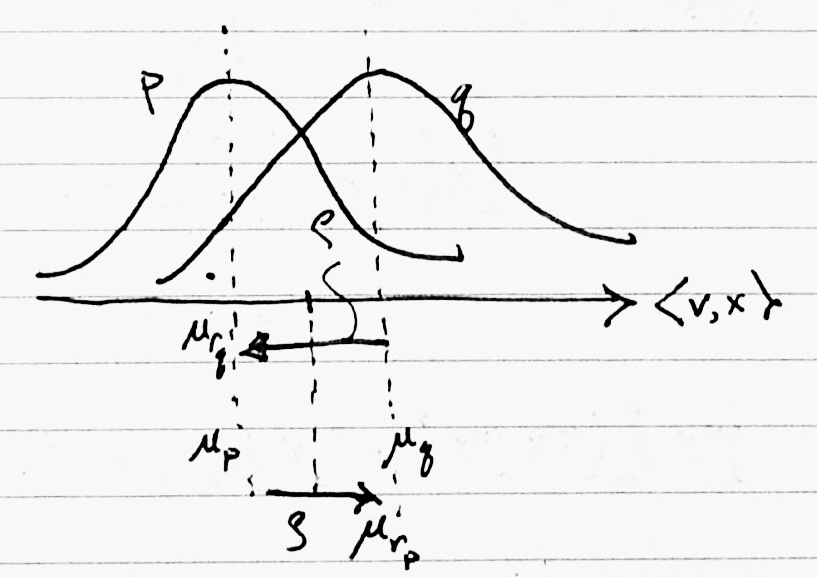
\includegraphics[width=0.4\textwidth]{figures/9-12-1.png}
    \end{center}
    \caption{
        Resilience allows us to perform an $\eps$-deletion to
        move from $\mu_p \to \mu_{r_p}$ and $\mu_q \to \mu_{r_q}$
        and pick up a factor of $+2 \rho$.
        Mean crossing allows us to relate $\mu_{r_p}$ and $\mu_{r_q}$.
    }
    \label{fig:resilience-mean-crossing}
\end{figure}

\begin{proof}[Proof of \nameref{lem:mean-crossing-property}]
    Consider \cref{fig:resilience-mean-crossing}, which visualizes the 1D
    projections of $p$ and $q$ in the $v$ direction.  To make $\braket{v,
    \mu_{r_q}}$ cross over $\braket{v, \mu_{r_p}}$, we would like to shift the
    mean of $q$ to the left and the mean of $p$ to the right as much as
    possible.  Thus, delete $\eps$ mass from the right tail of $q$ (and delete
    the left tail of $p$). Then
    \begin{align}
        \Pr_{r_p}[\braket{v,x} \geq \tau]
        \geq \frac{\Pr_{p}[\braket{v,x} \geq \tau]}{1 - \eps}
        \geq \frac{\Pr_{q}[\braket{v,x} \geq \tau] - \eps}{1 - \eps}
        = \Pr_{r_q}[\braket{v,x} \geq \tau]
    \end{align}
    where the first inequality is because $r_p$ is $p$ with the left
    tail deleted and renormalized by $1-\eps$,
    the second from
    $\Pr_q[\braket{v,x} \geq \tau] - \Pr_p[\braket{v,x} \geq \tau] \leq \widetilde{\TV}(p,q) \leq \eps$,
    and the third from $r_q$ being formed by deleting $\eps$ from the right tail of
    $q$ and renormalizing by $1-\eps$.

    We have shown that the right tail probabilities of $r_p$ are always larger
    than those of $r_q$, i.e. $r_p$ \emph{stochastically dominates} $r_q$.
    As a consequence, $\ex_{r_p}[\braket{v,x}] \geq \ex_{r_q}[\braket{v,x}]$.
\end{proof}

\begin{proof}[Proof of \cref{eq:9-12-desidirata-2}]
    Notice
    \begin{align}
        \widehat{\TV}_{\cH_{\lin}}(p,q)
        &= \sup_{v \in \RR^d, \tau \in \RR} \left\lvert
            \underbrace{\Pr_p[\braket{v,x} \geq \tau] - \Pr_q[\braket{v,x} \geq \tau]}_{\text{max discrepancy on halfspaces}}
        \right\rvert
    \end{align}
    By \nameref{thm:vc-inequality} and \myref{prop:vc-dim-half-spaces}
    \begin{align}
        \widehat{\TV}_{\cH_{\lin}}(\tilde{p}, \tilde{p}_n)
        &\leq O\left(\sqrt{\frac{vc(\text{half spaces})}{n}}\right)
        = O\left(\sqrt{\frac{d + \log \frac{1}{\delta}}{n}}\right)
    \end{align}
    with probability $\geq 1 - \delta$.
\end{proof}

\textbf{Consequences}:
\begin{itemize}
    \item For $(\rho, \eps + O(\sqrt{d/n}))$-resilient distributions, we can estimate mean with error $2 \rho$
    \item For bounded covariance, \cref{corr:mod-cont-cov} gave us
        $\rho(\eps) = O(\sqrt{\eps})$ hence
    \begin{align}
        L(p^*, \tilde{\theta}_{\widetilde{\TV}}(\tilde{p}_n)) 
        \leq O\left(\sqrt{\eps + \sqrt{d/n}}\right)
    \end{align}
    The lower bound $\sqrt{\eps}$ is what we get in the infinite sample $n \to \infty$
    limit, and $\sqrt{d/n}$ when $\eps \to 0$, so we would like $\sqrt{\eps} + \sqrt{d/n}$.
    The slack in the bound comes from $n \gg d / \eps^2$, whereas we would need $n \gg \frac{d}{\eps}$ but this analysis doesnt give it to us.

    \item For sub-Gaussians, $\rho(\eps) = O(\eps \sqrt{\log(1/\eps)})$.
    When $n \gg \frac{d}{\eps^2}$ we get $O(\eps \sqrt{\log (1/\eps)}$.
\end{itemize}
In general, this analysis holds for $n \gg d / \eps^2$: whenever this holds, we can
do as well as if we had infinite data. The analysis is tight in $d$ but loose in $\eps$.

\todo{$\widetilde{\TV}$ similar to Tukey median, may be useful for challenge problem}

\section{9/17/2019}

\subsection{Outline}

The \nameref{def:mdf} enjoys strong robustness bounds such
as \myref{prop:mdf-modulus-error-bound}. However, its definition
involves performing a projection onto $\cG$ (the set of distributions which
$p^*$ is assumed to be contained in):
\begin{align}
  \hat\theta(\tilde{p}) &= \theta^*(q) = \min_\theta L(q,\theta)
  \text{ where }q = \argmin_{q \in \cG} D(\tilde{p}, q)
\end{align}
We saw last time $D=\TV$ was not suitable if $\tilde{p} = \tilde{p}_n$ is discrete,
motivating the use of \nameref{def:tilde-tv}.
For bounded $k$th moments, we have that $\rho = \cO(\sigma_k \eps^{1 - 1/k})$
which under our previous theory (\cref{prop:mdf-tilde-tv} and \cref{eq:9-12-desidirata-2})
yields a guarantee
\begin{align}
  \|\mu(\tilde{p}_n) - \mu(p^*)\|_2 \leq \cO\left( \left(\underbrace{\eps + \sqrt{\frac{d}{n}}}_{\eps'}\right)^{1 - 1/k}\right)
\end{align}
whenever $\widetilde{\TV}_{\cH_{lin}}(\tilde{p}, p^*) \leq \eps$.

Today, we consider an alternative solution where we expand $\cG$ to some
larger set $\cM$ to perform the projection:
\begin{align}
  q = \argmin_{q \in \cM} \tilde{D}(\tilde{p}, q)
\end{align}
Under this analysis, we can achieve a tighter $\cO\left(\eps^{1 - 1/k} + \sqrt{d/n}\right)$ error.

Outline for today:
\begin{itemize}
  \item True ``empirical distribution''
  \item Expand the set idea
  \item Analyze concentration for bounded $k$th moments
    \begin{itemize}
      \item symmetrization
      \item truncated moments
      \item ledoux-talagrand
    \end{itemize}
\end{itemize}

\subsection{True Empirical Distribution}

Let $p_n^*$ define an empirical distribution drawn from $p^*$.

\begin{figure}[H]
\begin{center}
  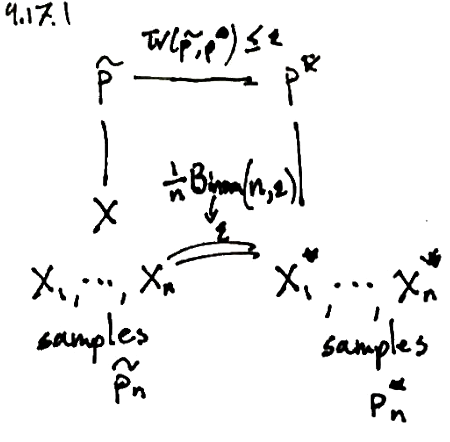
\includegraphics[width=0.3\textwidth]{figures/9-17-1.png}
\end{center}
\end{figure}


\textbf{Issue}: No overlap between $\tilde{p}_n$, $p_n^*$

\textbf{Solution}: Define \emph{coupling} between $p_n^*$ and $\tilde{p}_n$.

\begin{figure}[H]
\begin{center}
  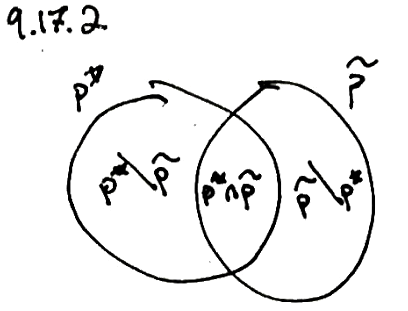
\includegraphics[width=0.3\textwidth]{figures/9-17-2.png}
\end{center}
\end{figure}

\begin{itemize}
  \item
    With probability $1 - \eps$:
    \begin{itemize}
      \item Sample from $p^* \cap \tilde{p}$, $X_i = \tilde{X_i} =$ sample
    \end{itemize}
  \item
    And with probability $\eps$:
    \begin{itemize}
      \item Sample $X_i^*$ from $p^* \setminus \tilde{p}$
      \item Sample $X_i$ from $\tilde{p} \setminus p^*$
    \end{itemize}
\end{itemize}

\textbf{Takeaway}:
$\underbrace{\TV(\tilde{p}_n, p_n^*)}_{\tilde{\eps}} \sim \frac{1}{n}\text{Binom}(n, \eps)$

\begin{lemma}[Tail bound for binomials]
  With probability $\geq 1 - \delta$
  \begin{align}
    \frac{1}{n} \text{Binom}(n, \eps)
    \leq O\left(\sqrt{\eps} + \sqrt{\frac{\log \frac{1}{\delta}}{2 n}}\right)^2
    = O\left(\eps + \frac{\log \frac{1}{\delta}}{2 n}\right)
  \end{align}
\end{lemma}

\begin{remark}
  This is tighter than Hoeffding, which would have given $\exp(-\eps^2 n / 3)$.
  Need Bernstein's inequality and Chernoff bound for binomial random variables
  to prove this.
\end{remark}

\subsection{Finite-Sample Concentration via Expanding the Set}%

\begin{figure}[H]
  \begin{center}
    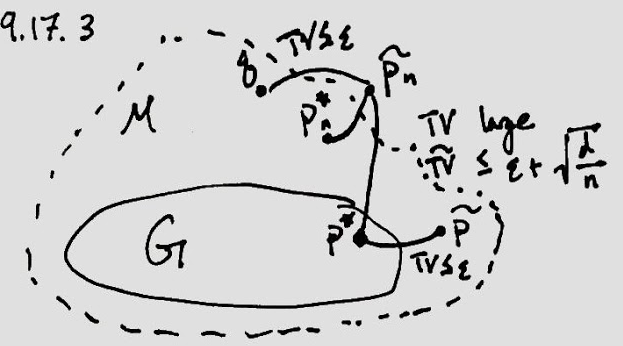
\includegraphics[width=0.5\textwidth]{figures/9-17-3.png}
    \caption{If we can expand $\cG \subset \cM$ so that $p_n^* \in \cM$,
      then we can form $q = \min_{q \in \cM} \TV(\tilde{p}_n, q)$ by projecting
      $\tilde{p}_n$ onto $\cM$ and use the ``true empirical distribution'' $p_n^*$
      to connect $q$ with $p^*$. This is made precise in \cref{prop:projection-bound-expand-G-to-M}}
  \end{center}
\end{figure}

Need three properties for $\cM$
\begin{itemize}
  \item $\cM$ large: $p_n^* \in \cM$ whp.
  \item $\cM$ small: modulus $\fm(\cM_{\eps})$ small
  \item $p_n^*$ good approx to $p^*$: $\|\mu(p^*) - \mu(p_n^*)\|_2$ bounded
\end{itemize}

\begin{proposition}\label{prop:projection-bound-expand-G-to-M}
  Suppose
  \begin{itemize}
    \item $p^*_n \in \cM$ wp $1 - \delta$
    \item $\TV(p_n^*, \tilde{p}_n) \leq \tilde{\eps}$ wp $1 - \delta$
  \end{itemize}
  Then projecting onto $\cM$ yields $q$ where
  \begin{align}
    \|\mu(q) - \mu(p^*)\|_2 \leq \fm(\cM, 2 \tilde{\eps}) + \|\mu(p^*) - \mu(p_n^*)\|_2
  \end{align}
  wp $1 - 2 \delta$.
\end{proposition}

\begin{proof}
  Since $p_n^* \in \cM$, we have
  \begin{align}
    \TV(\tilde{p}_n, q) &= \min_{q \in \cM} \TV(\tilde{p}_n, q) \leq \tilde{\eps}
  \end{align}
  Also by hypothesis $\TV(\tilde{p}_n, p_n^*) \leq \tilde{\eps}$, so
  by triangle inequality
  \begin{align}
    \TV(p_n^*, q) \leq 2 \tilde{\eps}
  \end{align}
  Together we have $\|\mu(p_n^*) - \mu(q)\|_2 \leq \fm(\cM, 2\tilde{\eps})$
  and by triangle inequality
  \begin{align}
    \|\mu(p^*) - \mu(q)\|_2 \leq \fm(\cM, 2 \tilde{\eps}) + \|\mu(p^*) - \mu(p_n^*)\|_2
  \end{align}
\end{proof}

\subsection{Expanding bounded kth moments to set of resilient distributions}

The following example will be our running example for this section.
We will see how bounded $k$th moments may require $n$ to be too large, and how
we can expand to the larger set of resilient distributions.

\begin{example}[Bounded $k$th moments]
  Consider distributions with bounded $k$th moments, that is
  \begin{align}
    \cG = \cG_k(\sigma)
    &= \{ p : \lvert \ex X \rvert_{\psi_k} \leq \sigma \} \\
    &= \{ p : \ex_p[ \lvert \braket{X - \mu, v} \rvert^k] \leq \sigma_k^k~\forall \|v\|_2 \leq 1\}
  \end{align}
  where $\psi_k(x) = x^k$.
  For example, $\cG_2(\sigma)$ are the distributions with bounded covariance.

  \textbf{Isuse}: $p_n^* \not\in \cG$ until $n \gg d^{k/2}$. For example,
  let $p^* = \cN(\mu, I)$, $p_n^* = \sum_{i=1}^n \frac{1}{n} \delta_{x_i}$,
  and notice for $v = \frac{x_1 - \mu}{\|x_1 - \mu\|}$
  we have $\|v\|_2 = 1$ but
  \begin{align}
    \ex_{p_n^*}[\lvert \braket{X - \mu, v}\rvert^k]
    \geq \frac{1}{n} \lvert \braket{x_1 - \mu, v}\rvert^k
    = \frac{1}{n} \underbrace{\|X_1 - \mu\|_2^k}_{=\cO(\sqrt{d})}
    &\asymp \frac{1}{n} d^{k/2} \\
    \ex_{p_n^*}[\lvert \braket{X - \mu, v}\rvert^k]^{1/k}
    &\asymp \left( \frac{1}{n} d^{k/2} \right)^{1/k}
    = \frac{\sqrt{d}}{n^{1/k}}
  \end{align}
  Asymptotically, we see that we need $n \gg d^{k/2}$ for the $k$th moments to
  remain bounded.

  \begin{figure}[H]
    \begin{center}
      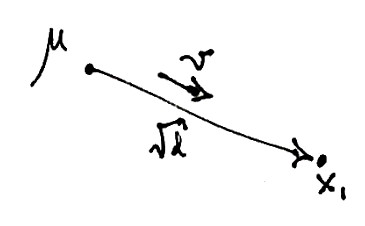
\includegraphics[width=0.3\textwidth]{figures/9-17-4.png}
    \end{center}
    \caption{The moment $\braket{X - \mu, v}$ along a
      single direction of a sample $v = \frac{x_1 - \mu}{\|x_1 - \mu\|}$
      is large, need to average over many samples before it washes out.}
  \end{figure}
\end{example}

Consider expanding bounded $k$th moments $\cG = \cG_k(\sigma)$ to the larger
set of resilient distributions $\cM = \cG_{\TV}(\rho, \eps)$ with $\rho = O(\eps^{1 - 1/k})$.
We already have a modulus bound $\fm(\cM, \eps) \leq 2 \rho = O(\eps^{1 - 1/k})$
from \myref{corr:mod-bound-resilient}, so
to make \cref{prop:projection-bound-expand-G-to-M} meaningful
it remains to show:
\begin{itemize}
  \item Bound 
    $\|\mu(p^*) - \mu(p_n^*)\|_2 = O\left(\sigma \sqrt{\frac{d}{n} \delta^{-1/k}}\right)$
    We do this using Kintchine's inequality.

  \item $p^*_n \in \cM$ whp. 
    We do this using truncated moments.
\end{itemize}

\begin{lemma}
  \begin{align}
    \|X\|_2 &= \ex_{v \sim \cN(0,I)}[\lvert\braket{x,v}\rvert] \sqrt{\frac{\pi}{2}}
  \end{align}
\end{lemma}
\begin{proof}
  \begin{align}
    \ex[\lvert
    \braket{
      (\|x\|_2, 0, \ldots, 0),
      (v_1,\ldots, v_d)
    } \rvert]
    = \ex[\lvert v_1 \rvert \cdot \|x\|_2] \\
    \ex[\lvert v_1\rvert] = \sqrt{2/\pi}
  \end{align}
\end{proof}

\begin{remark}
  There's a better version of the above called \emph{Khintchine's inequality}:
  \begin{align}
    \|X\|_2 \leq \sqrt{2} \ex[\lvert \braket{X, \eps} \rvert]
  \end{align}
  with $\eps \sim \text{Rad}$. So we can just test using Rademachers rather
  than Gaussian process.
\end{remark}

\todo{We failed to prove the second easy thing in class using above, see next lecture for resolution}

\subsubsection{Truncated moments}

Now we show $p_n^* \in \cM$, introducing some new ideas along the way.

\textbf{Problem}: $\| \cdot \|_{\psi_k}$ is not small.

\textbf{Solution}: Truncate moments, replace $\psi_k(x) = x^k$ with
\begin{align}
  \tilde{\psi}_k(x) = \begin{cases}
    x^k & x \leq x_0 \\
    k x_0^{k-1} (x - x_0) + x_0^k & x > x_0
  \end{cases}
\end{align}
This is equal to $\psi_k$ for $x \leq x_0$ and linearly interpolates beyond $x \geq x_0$.

\begin{figure}[H]
  \begin{center}
    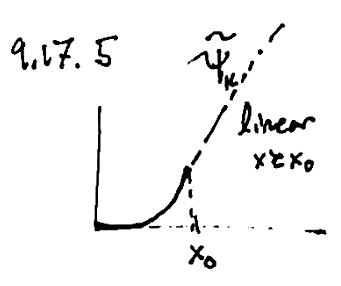
\includegraphics[width=0.3\textwidth]{figures/9-17-5.png}
  \end{center}
  \caption{The Orlicz function $\tilde{\psi}_k$ used for truncating moments}
  \label{fig:tilde-psi-k}
\end{figure}

$\tilde{\psi}_k$ is $L$-Lipschitz with $L = k x_0^{k-1}$, so in particular
if we choose $x_0 = \left(\frac{1}{\eps}\right)^{1/k}$ then we have $L = k / \eps^{1 - 1/k}$.

\begin{proposition}\label{prop:truncated-moments-bound}
  Let $X_1, \ldots, X_n \sim p^*$, where $p^* \in \cG_k(\sigma)$. Then
  \begin{align}
    \ex_{X_i \sim p^*}\left[
      \sup_{\|u\|_2 = 1} \frac{1}{n} \sum_{i=1}^n \tilde{\psi}_k\left(
        \left\lvert \frac{\braket{X_i - \mu, v}}{\sigma}\right\rvert
      \right)
    \right]
    &\leq 1 + 2 L \sqrt{\frac{d}{n}}
  \end{align}
  where $L = k x_0^{k-1}$.
\end{proposition}

\begin{remark}
  When  $n \geq 4 L^2 d = 4 k^2 d / \eps^{2 - 2/k}$, we have
  \begin{align}
    \sup_{\|u\|_2 = 1} \frac{1}{n} \sum_{i=1}^n \tilde{\psi}_k\left(
      \left\lvert \frac{\braket{X_i - \mu, v}}{\sigma}\right\rvert
    \right)
    \leq 2
  \end{align}
  This implies that $p_n^*$ has bounded Orlicz norm
  $\|p_n^*\|_{\tilde{\psi}_k}$, so by \cref{lem:orlicz-norm-resilient}
  $p_n^*$ is resilient with parameter $\sigma \eps \tilde{\psi}^{-1}(2/\eps)$.
  So we really need to control how fast $\sigma \eps \tilde{\psi}^{-1}(2/\eps)$
  grows. From \cref{fig:bound-tilde-psi-k-inv}, we may conclude
  \begin{align}
    \sigma \eps \tilde{\psi}^{-1}(2/\eps)
    \leq 2 \sigma \eps \underbrace{\left(\frac{1}{\eps}\right)^{1/k}}_{> 0}
    = 2 \sigma \eps^{1 - 1/k}
  \end{align}


  \begin{figure}[H]
    \begin{center}
      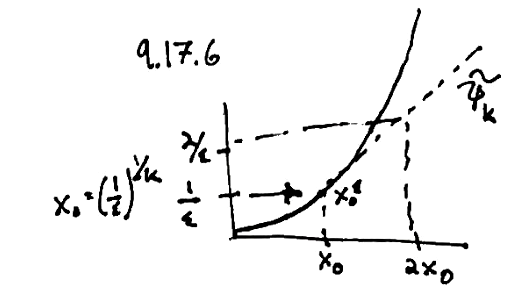
\includegraphics[width=0.4\textwidth]{figures/9-17-6.png}
    \end{center}
    \caption{A proof by picture why $\psi^{-1}(2/\eps) \leq 2 x_0 = 2 \eps^{-1/k}$}
    \label{fig:bound-tilde-psi-k-inv}
  \end{figure}

\end{remark}

\subsubsection{Ledoux-Talagrand contraction}%
\label{ssec:ledoux-talagrand-first}

This result is used as part of symmetrization arguments. If I have already symmetrized and I have
a Lipschitz function, than I can always repalce the function with just its
arguments and make things bigger.

\begin{theorem}[Ledoux-Talagrand]
  \begin{align}
    \ex_{\eps}\left[
      \sup_{v \in V} \frac{1}{n} \sum^{n}_{i=1} \eps_i \phi(\braket{x_i, v})
    \right]
    \leq \ex_\eps\left[
      \sup_{v \in V} \frac{1}{n} \sum_{i=1}^n \eps_i \braket{x_i, v}
    \right]
  \end{align}
  for $\phi$ $1$-Lipschitz, i.e. $\vert \phi(x) - \phi(y) \rvert \leq \lvert x - y \rvert$,
  $V$ a symmetric set, and $\eps \sim \text{Rad}$.
\end{theorem}

\begin{proof}[Proof of \cref{prop:truncated-moments-bound}]
  \begin{align}
    \ex_{X_i \sim p^*}\left[
      \sup_{\|u\|_2 = 1} \frac{1}{n} \sum_{i=1}^n \tilde{\psi}_k\left(
        \left\lvert \frac{\braket{X_i - \mu, v}}{\sigma}\right\rvert
      \right)
    \right]
    = \underbrace{\ex[\tilde{\psi}]}_{\leq \ex\psi \leq 1} + \sup_{\|v\|_2 \leq 1} \frac{1}{n} \sum^{n}_{i=1} \left(
      \tilde{\psi}_k(\lvert \braket{x_i - \mu, v} / \sigma \rvert) - \ex[\tilde\psi]
    \right)
  \end{align}

  Symmetrize?
  \begin{align}
    \ex_{X_i, X_i' \sim p^*, \eps \sim \text{Rad}}\left[
      \sup_{\|v\|_2 \leq 1} \frac{1}{n} \sum^{n}_{i=1}
      \eps_i \left(
        \tilde{\psi}_k\left(\frac{\lvert \braket{X_i - \mu, v}\rvert}{\sigma}\right)
        -  \tilde{\psi}_k\left(\frac{\lvert \braket{X_i' - \mu, v}\rvert}{\sigma}\right)
      \right)
    \right]
  \end{align}
  \todo{See next lecture}
\end{proof}

\section{9/19/2019: Ledoux-Talagrand and Truncated Moments}

\subsection{Recap}

\begin{itemize}
  \item Expand $\cG$ to $\cM$
    \begin{itemize}
      \item Bound modulus of $\cM$
      \item Show $p_n^* \in \cM$
      \item Bound $\|\mu(p_n^*) - \mu(p^*)\|_2$
    \end{itemize}
  \item $\cG = \cG_k(\sigma) =$ bounded $k$th moments
    (needed $n \geq d^{k/2}$ samples if $\cM = \cG$)
  \item $\cM = \cG_{\TV}(\rho, \eps) =$ $(\rho, \eps)$-resilient distributions
    with $\rho - \cO(\sigma \eps^{1 - 1/k})$
\end{itemize}

\subsection{Truncated moments bounds}

Our strategy to show $p_n^* \in \cM$ is to consider the truncated (Orlicz)
function
\begin{align}
  \tilde{\psi}_k &= \begin{cases}
    x^k &\text{if } x \leq x_0 \\
    k x_0^{k-1} (x - x_0) + x_0^k&\text{if } x > x_0
  \end{cases}
\end{align}
This function behaves as $x^k$ until $x=x_0$, after which it is linear.
Note that $\tilde{\psi}_k$ is $L$-Lipschitz with $L = k x_0^{k-1}$.

\textbf{Todo this lecture:}
\begin{itemize}
  \item Ledoux-Talagrand
  \item Bound $\|\mu(p_n^*) - \mu(p^*)\|_2$ via Khintchine and Rosenthal
  \item Show truncated moments $\tilde{\psi}$ concentrate
\end{itemize}

\begin{definition}[Stochastic Dominance]
  Let $Y, Z$ be RVs on $\RR$.
  $Z$ \emph{1st-order stochastically dominates} $Y$ if
  \begin{align}
    \ex[f(Z)] \geq \ex[f(Y)]
  \end{align}
  for all increasing $f$.

  \textbf{Intuition}: $Y \mapsto Z$ by moving CDF to the right:

  Figure 9.19.1

\end{definition}

\begin{lemma}
  Let $Y$ have probability $1/2$ of $y_1$ or $y_2$ ($y_1 \leq y_2$)
  and $Z$ same for $z_1 \leq z_2$.

  Thten $Z$ stochastically (1st order) dominates $Y$ iff $y_1 \leq z_1$
  and $y_2 \leq z_2$.
\end{lemma}

\begin{proof}
  Fig 9.19.2
  \begin{align}
    \ex[f(Y)] &= 1 \\
    \ex[f(Z)] &\leq \frac{1}{2} \\
  \end{align}

  For the sufficiency,
  \begin{align}
    \ex[f(Z)]
    &= \frac{f(z_1) + f(z_2)}{2}
    \geq \frac{f(y_1) + f(y_2)}{2}
    = \ex[f(Y)]
  \end{align}
\end{proof}

\begin{definition}[Second order stochastic dominance]
  $Z$ \emph{2nd-order stochasttically dominates} $Y$ if
  \begin{align}
    \ex[g(Y)] \leq \ex[g(Z)]
  \end{align}
  for all convex, increasing $g$

  \textbf{Intuition}: $Y \mapsto Z$ by pushing to right and spreading out
\end{definition}

\begin{lemma}\label{lem:two-point-2o-sd}
  Let $Y$ have probability $1/2$ being $y_1$ or $y_2$ and same for $Z$.
  If
  \begin{align}
    \frac{1}{2}(y_1 + y_2) &\leq \frac{1}{2}(z_1 + z_2) \\
    z_2 &\geq y_2
  \end{align}
  then $Z \preceq Y$.
\end{lemma}

\begin{proof}
  Figure 9.17.3
\end{proof}

\begin{theorem}[Ledoux-Talagrand]
  Let $\phi : \RR \to \RR$ $L$-Lipschitz, $\phi(0) = 0$,
  $\{\eps_i\}_{i=1}^n \simiid \Rad$, $T =$ set of $n$-tuples $(t_1,\ldots,t_n)$
  (think $t_i = \braket{X_i - \mu, v}$). Then
  \begin{align}
    \ex\left[g \left(
        \sup_{t \in T} \sum_{i=1}^n \eps_i \phi(t_i)
    \right)\right]
    &\leq \ex\left[
      g\left(
        \sup_{t \in T} L \sum_{i=1}^n \eps_i t_i
      \right)
    \right]
  \end{align}
  for all convex increasing $g$.
\end{theorem}

In terms of stochastic dominance, this is saying that the random variables
\begin{align}
  Y &= \sup_{t \in T} \sum_{i=1}^n \eps_i \phi(t_i) \\
  Z &= \sup_{t \in T} L \sum_{i=1}^n \eps_i t_i
\end{align}
satisfy the second order stochastic dominance $Z \succeq Y$.
This means that $Z$ is more ``spread out'' than $Y$, which makes sense because
$\lvert \phi(s) - \phi(t) \rvert \leq L \lvert s - t \rvert$.

Another way to get this intutiion is to notice that the term inside the
supremum (for $L = 1$, if $\eps_i$ were Gaussian)
\begin{align}
  \Var\left(\sum_{i} \eps_i \phi(t_i)\right)
  &= \sum_i \phi(t_i)^2
  \leq \sum_{i} \lvert t_i \rvert^2
  = \Var\left(\sum_i \eps_i t_i\right)
\end{align}
So we would expect $Z$ to be more ``spread out'' because it has greater
variance.

\begin{proof}[Proof for $n=2$]
  Let $T$ be the set of pairs $(a,b)$, $\phi$ be $1$-Lipschitz.
  Need to show
  \begin{align}
    \ex_\eps\left[
      g\left(
        \underbrace{\sup_{(a,b) \in T} a + \eps \phi(b)}_{\eqqcolon Y}
      \right)
    \right]
    &\leq
    \ex_\eps\left[
      g\left(
        \underbrace{\sup_{(a,b) \in T} a + \eps b}_{\eqqcolon Z}
      \right)
    \right]
  \end{align}
  Let $(a_+, b_+)$ be the maximizer of $a + \phi(b)$, and
  $(a_-, b_-)$ the maximizer of $a - \phi(b)$. Then
  \begin{align}
    \Pr[Y = y_1 = a_+ + \phi(b_+)] &= 1/2 \\
    \Pr[Y = y_2 = a_- - \phi(b_-)] &= 1/2 \\
    \Pr[Z = z_1 = \max(a_+ + b_+, a_- + b_-)] &= 1/2 \\
    \Pr[Z = z_2 = \max(a_- - b_-, a_+ + b_-+)] &= 1/2
  \end{align}

  Fig 9.19.4

  By Lipschitz condition and definition of $y_i$, $z_i$:
  \begin{align}
    \max(y_1, y_2) &\leq \max(z_1, z_2) \\
    \max(a_+ + \phi(b_+), a_- - \phi(b_-))
                   &\leq \max(a_+ + \lvert b_+ \rvert, a_- + \lvert b_- \rvert) \\
    y_1 + y_2 &\leq z_1 + z_2 \\
    a_+ + a_- + \phi(b_+) - \phi(b_-)
              &\leq a_+ + a_- + \lvert b_+ - b_- \rvert
  \end{align}
  By \cref{lem:two-point-2o-sd}, we are done.
\end{proof}

\begin{proof}[Extending to $n > 2$]
  \begin{align}
    \ex_{\eps_{1:n}}\left[
      g \left(
        \sup_{t \in T} \sum_{i=1}^n \eps_i \phi(t_i)
      \right)
    \right]
    &=
    \ex_{\eps_{1:n-1}} \left[
      \ex_{\eps_{n}}\left[
        g \left(
          \sup_{t \in T} \underbrace{\sum_{i=1}^{n-1} \eps_i \phi(t_i)}_{a} + \eps_n \phi(\underbrace{t_n}_{b})
        \right)
      \middle\vert \eps_1,\ldots, \eps_{n-1} \right]
    \right] \\
    &\leq
    \ex_{\eps_{1:n-1}} \left[
      \ex_{\eps_{n}}\left[
        g \left(
          \sup_{t \in T} \sum_{i=1}^{n-1} \eps_i \phi(t_i) + \eps_n t_n
        \right)
      \middle\vert \eps_1,\ldots, \eps_{n-1} \right]
    \right] \\
    &=
    \ex_{\eps_{1:n}} \left[
      g \left(
        \sup_{t \in T} \sum_{i=1}^{n-1} \eps_i \phi(t_i) + \eps_n t_n
      \right)
    \right] \\
    &=
    \ex_{\eps_{[n] \setminus \{n-1\}}} \left[
        \ex_{\eps_{n-1}}\left[
          g \left(
            \sup_{t \in T} \sum_{i \in [n] \setminus \{n-1, n\}} \eps_i \underbrace{\phi(t_i) + \eps_n t_n }_{a}
            + \underbrace{\eps_{n-1} \phi(t_{n-1})}_{b}
          \right)
        \middle\lvert \eps_{[n] \setminus \{n-1\}} \right]
      \right]
  \end{align}
\end{proof}


\textbf{Goal}: Bound $\|\hat{\mu}_n - \mu\|_2$

Problem last time:
\begin{align}
  \ex[ \|\hat{\mu}_n - \mu\|_2^k ]
  &= \ex[ \| \frac{1}{n} \sum_{i=1}^n (X_i - \mu)\|_2^k ]
\end{align}
One way to handle the norm is to take a supremum over inner products with
$v \in \cS^{d-1}$. Another is to use decouopling:

\textbf{Decoupling technique}: Use Khintchine's inequality to add in
an $\ex_\eps$. Symmetrization would have added random sign variables across
$n$ (one for each pair $(X_i, X_i')$), here we are addding random sign
variables across $d$.

\begin{lemma}[Khintchine's inequality]
  Let $\eps = (\eps_1, \ldots, \eps_n) \simiid \Rad$.
  \begin{align}
    A_k \|Z\|_2 \leq \ex_\eps[\lvert \braket{\eps,z}\rvert^k]^{1/k} \leq B_k \|Z\|_2
  \end{align}
  with $A_k = \Theta(1)$ and $B_k = \Theta(\sqrt{k})$ if $k \geq 1$.
\end{lemma}

Proceeding
\begin{align}
  \ex_X [ \|\hat{\mu}_n - \mu\|_2^k ]
  &= \ex_X [ \| \frac{1}{n} \sum_{i=1}^n (X_i - \mu)\|_2^k ] \\
  &\overset{?}{=} \ex_{X,\eps} [ \lvert \braket{\frac{1}{n} \sum_{i=1}^n (X_i - \mu), \eps} \rvert^k ] \\
  &\leq \cO(1)^k \ex_{X, \eps}\left[
    \left\lvert
      \frac{1}{n} \sum^{n}_{i=1} \underbrace{\braket{X_i - \mu, \eps}}_{\eqqcolon z_i}
    \right\rvert^k
  \right]
\end{align}
Now pulling out the $n^{-k}$ and applying Rosenthal's inequality
\begin{align}
  \ex[\lvert \sum_i z_i \rvert^k]
  &\leq \cO(k)^k \sum_i \ex[\lvert Z_i \rvert^k]
  + \cO(\sqrt{k})^k \left(\sum_i \ex[\lvert Z_i \rvert^2]\right)^{k/2}
\end{align}
Under bounded $k$th moments hypothesis, $\ex[\lvert \braket{X - \mu,
v}\rvert^k] \leq \sigma^k \|v\|_2^k$ so
\begin{align}
  \ex[\lvert Z_i \rvert^k]
  &= \ex_{X,\eps}[\lvert \braket{X_i - \mu, \eps}\rvert^k]
  \leq \ex_\eps[\|\eps\|_2^k \sigma^k]
  = d^{k/2} \sigma^k
\end{align}

To record a tighter bound (since typically $\sigma_k \approx \sqrt{k} \sigma_2$),
let
\begin{align}
  \ex[\lvert \braket{X - \mu, v}\rvert^k]
  &\leq \sigma_k^k \|v\|_2^k \\
  \ex[\lvert \braket{X - \mu, v}\rvert^2]
  &\leq \sigma_2^k \|v\|_2^2
\end{align}
So Rosenthal's inequality (and adding back $n^{-k}$) becomes
\begin{align}
  \ex[\|\hat{\mu}_n - \mu\|_2^k]
  &\leq \cO(1)^k \ex_{X, \eps}[\lvert \frac{1}{n} \sum^{n}_{i=1} \braket{X_i - \mu, \eps}\rvert^k] \\
  &\leq \cO(1/n)^k \left[
    \cO(k)^k n d^{k/2} \sigma_k^k + \cO(\sqrt{k})^k (n d^{1/2} \sigma_2^2)^{k/2}
  \right] \\
  &= \cO\left(
    \left( \frac{k \sqrt{d}}{n} \sigma_k\right)^k n
    + \left(\sqrt{\frac{k d}{n}}\sigma_2 \right)^k
  \right)
\end{align}
In the case $\sigma_k = \sqrt{k} \sigma_2$, the second term dominates as long
as $n \geq k^{2k / (k-2)}$.

\textbf{Takeaway}: The average deviation $\ex[\|\hat{\mu}_n - \mu\|_2^k]^{1/k} \approx \cO(\sqrt{k d / n} \sigma_2)$.


\subsection{Tying back to what we acre}

\textbf{Goal}: we want the following to concentrate
\begin{align}
  \ex\left[\left\lvert
      \sup_{\|v\|_2 \leq 1} \frac{1}{n} \sum_{i=1}^n \left(
        \tilde{\psi}_k\left(\left\lvert
            \frac{\braket{X_i - \mu, v}}{\sigma}
          \right\rvert\right)
      \right)
      - \mu_{\tilde{\psi}_k}(v)
    \right\rvert^k\right]
\end{align}

By symmetrization
\begin{align}
  \ex\left[\left\lvert
      \sup_{\|v\|_2 \leq 1} \frac{1}{n} \sum_{i=1}^n \left(
        \eps_i \tilde{\psi}_k\left(\left\lvert
            \frac{\braket{X_i - \mu, v}}{\sigma}
          \right\rvert\right)
      \right)
    \right\rvert^k\right]
\end{align}

By Ledoux with $g(x) = x^k$
\begin{align}
  \ex\left[\left\lvert
      \sup_{\|v\|_2 \leq 1} \frac{1}{n} \sum_{i=1}^n \left(
        \eps_i \frac{(X_i - \mu)}{\sigma}
      \right)
    \right\rvert^k\right]
\end{align}
By a stronger version of the mean deviation inequality we just proved

\section{9/24/2019}

\begin{itemize}
  \item PSet 2 posted by Friday, due Tuesday 10/8
\end{itemize}

\subsection{Recap}%

Wanted to bound truncated moments $\tilde{\psi}_k$
\begin{itemize}
  \item Ledoux-Talagrand for bounding deviation of $\tilde{\psi}_k$
  \item Khintchin and Rosenthal to bound $\ex[\|\hat\mu_n - \mu\|_2^k]$
\end{itemize}

Today
\begin{itemize}
  \item Finish up proof
  \item Efficient algorithms for $\cG_{cov}(\sigma)$
\end{itemize}

\textbf{Goal}: Bound
\begin{align}
  \sup_{\|v\| \leq 1} \frac{1}{n}
  \sum_{i=1}^n \tilde{\psi}_k\left(\left\lvert \frac{\braket{x_i - \mu, v}}{\sigma}\right\rvert\right),
  \quad\text{ where }
  \tilde{\psi}_k(x) = \begin{cases}
    x^k, &\text{ if }x \leq x_0\\
    \text{linear}, &\text{ ow }
  \end{cases}
  \text{ is $L$-Lipschitz.}
\end{align}

For convenience, take $\mu = 0$ and $\sigma = 1$.

Consider symmetrizing:
\begin{align}
  \underbrace{\sup_{\|v\|_2 \leq 1} \frac{1}{n} \sum_{i=1}^n \tilde{\psi}_k(\lvert \braket{x_i, v}\rvert) - \ex_{X'}[\tilde{\psi}_k(\lvert \braket{x_i', v}\rvert)]}_{Z(X)} + 1
\end{align}
We're going to bound $Z(X)$ using Chebyshev's inequality.

Let $g$ be convex increasing.
\begin{align}
  \ex_X[g(Z(X))]
  &= \ex_X g\left(\sup_{\|v\|_2 \leq 1} \frac{1}{n} \sum_{i=1}^n \tilde\psi_k(\braket{x_i, v}) - \underbrace{\ex_{X'} \tilde\psi_k(\braket{x_i', v})}_{\sup \ex \leq \ex \sup} \right) \\
  &\leq \ex_X g\left(\ex_{X'} \sup_{\|v\|_2 \leq 1} \frac{1}{n} \sum_{i=1}^n \tilde\psi_k(\braket{x_i, v}) - \tilde\psi_k(\braket{x_i', v}) \right) \\
  &\leq \ex_{X,X'} g\left(\sup_{\|v\|_2 \leq 1} \frac{1}{n} \sum_{i=1}^n \tilde\psi_k(\braket{x_i, v}) - \tilde\psi_k(\braket{x_i', v}) \right) \\
  &= \ex_{X,X',\eps} g\left(\sup_{\|v\|_2 \leq 1} \frac{1}{n} \sum_{i=1}^n \eps(\tilde\psi_k(\braket{x_i, v}) - \tilde\psi_k(\braket{x_i', v})) \right) \\
  &\leq \ex_{X,X',\eps} g\left(
    \underbrace{\sup_{\|v\|_2 \leq 1} \frac{1}{n}\sum_{i=1}^n
    \eps \tilde\psi_k(\braket{x_i, v})}_A
    + \underbrace{\sup_{\|v\|_2 \leq 1} \frac{1}{n}\sum_{i=1}^n
    \eps\tilde\psi_k(\braket{x_i', v'})}_B
\right)
\end{align}
Applying Jensen's on $g$ gigves $\ex[\cdot] \leq \ex[g(2A)]$ so
\begin{align}
  \ex_X[g(Z(X))]
  &\leq \ex_{X,\eps} g\left(\sup_{\|v\|_2 \leq 1} \frac{2}{n} \sum_{i=1}^n \eps\tilde\psi_k(\braket{x_i, v}) \right)
\end{align}
Since $\tilde\psi_k$ is $L$-Lipschitz, applying Ledoux-Talagrand gives
\begin{align}
  \ex_X[g(Z(X))]
  &\leq \ex_{X,\eps} g\left(\sup_{\|v\|_2 \leq 1} \frac{2 L}{n} \sum_{i=1}^n \eps_i\braket{x_i, v} \right) \\
  &= \ex_{X,\eps} g\left(\sup_{\|v\|_2 \leq 1} \braket{x_i, \frac{2 L}{n} \sum_{i=1}^n \eps_i v} \right) \\
  &= \ex_{X,\eps} g\left(\left\|\frac{2 L}{n} \sum_{i=1}^n \eps_i v\right\|_2 \right)
\end{align}
So far this has been for generic convex increasing $g$.
For $k$th moments, $g(x) = x^k$ and
\begin{align}
  \ex_X[g(Z(X))]
  &\leq \left(\frac{2 L}{n}\right)^k
  \ex_{X,\eps} \left[\left\|
    \sum_{i=1}^n \eps_i X_i\|_2^k
  \right\|\right]
\end{align}
The remainder is handled using Khintchine and Rosenthal's inequality.

\subsection{Efficient algorithms via eigenvector projection}%

Let the true distribution $p^* \in \cG_{cov}(\sigma)$, so $\|\Cov_{p^*}[X]\| \leq \sigma^2$.
Let the corrupted distribution $\tilde{p}$ be such that $\TV(p^*, \tilde{p}) \leq \eps$.

\textbf{Goal}: Estimate $\mu = \ex_{p^*}[X]$ with error
$\cO(\sigma \sqrt{\eps})$ in $\ell_2$-norm.

\textbf{Will show}: There exists an efficient algorithm that outputs $q$ such that:
\begin{itemize}
  \item $\TV(q, p^*) = \cO(\eps)$, which yields a modulus of continuity bound
  \item $\|\Cov_q(X)\| = \cO(\sigma^2)$, which yields an error $\cO(\cO(\sigma) \sqrt{\cO(\eps)}) = \cO(\sigma\sqrt{\eps})$.
\end{itemize}

\subsubsection{Representation}%

Let $\tilde{p}$ be the empirical distribution over $n$ points
$\{x_i\}_{i=1}^n$.

Let $p^*$ be the empirical distribution over a subset $\{X_i\}_{i \in S}$ of
points from $\tilde{p}$ with $\lvert S \rvert \geq (1 - \eps)n$.

\begin{itemize}
  \item Empirical distribution, so we can store on computer
  \item Subset condition, which is equivalent to
    $p^*$ being an $\eps$-deletion of $\tilde{p}$,
    hence $\TV(p^*, \tilde{p}) \leq \eps$
  \item Deleting points can't make $\Cov[X]$ large: for
    any $q$ an $\eps$-deletion of $p$
    \begin{align}
      \Cov_q[X] \preceq \frac{1}{1-\eps} \Cov_p[X]
    \end{align}
\end{itemize}

Figure 9.24.1: We had bad examples previously by putting all
the points in a single direction.

\textbf{Algorithm}:
\begin{itemize}
  \item Initialize $c_i = 1$ for all $i$
  \item Let $q(c)$ be the weight $\frac{c_i}{\sum_j c_j}$ on point $x_i$
  \item Repeat:
    \begin{itemize}
      \item Compute $\hat\mu_ = \ex_{q(c)}[X]$
      \item Compute $\hat\Sigma_c = \Cov_{q(c)}[X]$
      \item Let $\hat\sigma_c^2
        = \sup_{\|v\| \leq 1} v^\top \hat\Sigma_c v
        = \sup_{\|v\|_2 \leq 1} \frac{
          \sum_{i=1}^n c_i \braket{x_i - \hat\mu_c, v}^2
        }{\sum_i c_i}$,
      \item If $\hat\sigma_c^2 \leq 20 \sigma^2$, output $q(c)$
      \item Else, $c_i \leftarrow c_i \left(1 - \frac{\tau_i}{\tau_{\max}}\right)$, $\tau_i = \braket{x_i - \hat\mu_c, v^*}^2$, $\tau_{\max} = \max_i \tau_i$.
    \end{itemize}
\end{itemize}

The algorithm is based on the intuition that
the maximizing $v^*$ for $v^\top \Sigma v$ is precisely
the top eigenvector for $\Sigma$.

\textbf{Intuition}: If $\mu \approx \hat\mu$, then
$\tau_i \approx \braket{x_i - \mu, v^*}^2$ is the projection
onto $v^*$.

Figure 9.24.2

However this intuition is flawed in two ways:
\begin{itemize}
  \item Assuming $\mu \approx \hat\mu_c$, which is the goal to begin with
  \item Only holds in expectation (c.f. downweighting)
  \item Not many bad points
\end{itemize}

\begin{proposition}
  Suppose $\|\Cov_{p^*}[X]\|\leq \sigma^2$.
  Then Algorithm outputs $q$ such that
  \begin{itemize}
    \item $\TV(p^*, q) \leq \frac{\eps}{1-\eps}$
    \item $\|\Cov_q[X]\| \leq 20 \sigma^2$
  \end{itemize}
  Hence by modulus bound, $\|\mu(q) - \mu\|_2 = O(\sigma\sqrt{\eps})$
\end{proposition}

\begin{proof}[Sketch of proof]
  Invariant 1: $\TV(p^*, q(c)) \leq \frac{\eps}{1-\eps}$ always.

  Invariant 2: $\sum_{i \in S} (1 - c_i) \leq \sum_{i \not\in S}(1 - c_i)$

  The second implies the first.

  Let $c_i' = c_i \left( 1 - \frac{\tau_i}{\tau_{\max}} \right)$.
  \begin{align}
    \sum_{i \in S} (1 - c_i') = \sum_{i \in S} (1 - c_i) +
    \underbrace{\sum_{i \in S} (c_i - c_i')}_{=\frac{1}{\tau_{\max}} \sum_i c_i \tau_i}
  \end{align}
  To show Invariant 2, want
  \begin{align}
    \sum_{i \in S} c_i \tau_i &\leq \sum_{i \not\in S} c_i \tau_i
  \end{align}
  Note
  \begin{align}
    \sum_{i \in S} c_i \tau_i
    &= \sum_{i \in S} c_i \braket{x_i - \hat\mu_c, v^*}^2
    \leq \underbrace{\left(\frac{1}{\lvert S \rvert} \sum_{i \in S} \braket{x_i - \hat\mu_c, v^*}^2\right)}_{\text{looks like covariance}}
  \cdot (1 - \eps)n
  \end{align}
  Expanding this term
  \begin{align}
    \frac{1}{\lvert S \rvert} \sum_{i \in S} \braket{x_i - \hat\mu_c, v^*}^2
    &= (v^*)^\top \ex_{p^*}[(X - \hat\mu_c) (X - \hat\mu_c)^\top] v^* \\
    &= (v^*)^\top \left(
      \Cov_{p^*}[X] + (\mu - \hat\mu_c)(\mu - \hat\mu_C)^\top
    \right) v^* \\
    &= \underbrace{(v^*)^\top \Cov_{p^*}[X] v^*}_{\leq \sigma^2}
    + \underbrace{\braket{v^*, \mu - \hat\mu_c}^2}_{\leq \|\mu - \hat\mu_c\|_2^2
    \leq \cO(\hat\sigma_c^2 \underbrace{\TV(p^*, q(c))}_{\leq \eps/(1-\eps)}}
  \end{align}
  Therefore
  \begin{align}
    \sum_{i \in S} c_i \tau_i &\leq (1 - \eps) n (\sigma^2 +
    \underbrace{\cO(\hat\sigma_c^2 \eps)}_{\text{small as }\eps \to 0})
  \end{align}
  \begin{align}
    \sum_{i=1}^n c_i \tau_i
    &= \hat\sigma_c^2 \underbrace{\left(\sum_{i=1}^n c_i\right)}_{\geq (1 - 2 \eps) n}
  \end{align}

  \textbf{Want}: $\sum_{i=1}^n c_i \tau_i \geq 2 \sum_{i \in S} \underbrace{c_i \tau_i}_{\approx \sigma^2} \approx 20 \sigma^2$ where 20 works if $\eps \leq 1/12$.
\end{proof}

\textbf{Generic proof outline for efficient algorithms}: $\tau_i$ measures how bad points are, downweight on the $\tau_i$.

\section{9/26/2019}

\subsection{Recap}%

\begin{itemize}
  \item Efficient algorithms for $\cG_{cov}(\sigma)$
  \item Project onto top eigenvectors
    \begin{itemize}
      \item Revealed bad points
    \end{itemize}
  \item Invariant 1: remove more bad than good points
  \item \textbf{TODO} Invariant 2: $\TV(q(c), p^*) \leq \frac{\eps}{1-\eps}$
  \item Today:
    \begin{itemize}
      \item Other norms
        \begin{itemize}
          \item Dual norm
          \item Approximate eigenvector via SDP
          \item Grothendieck's inequality
        \end{itemize}
    \end{itemize}
\end{itemize}

Recall our algorithm, which $\tilde{p}$ is an empirical
distribution over $n$ points $\{x_1, \ldots, x_n\}$ and
$p^*$ an empirical distribution over a subset $\{x_i\}_{i \in S}$
from $\tilde{p}$ with $\lvert S \rvert \geq (1 - \eps) n$.
Our algorithm represented the distribution $q$ as
\begin{align}
  q(c) : \text{ place }\frac{c_i}{\sum_{i=1}^n c_i}\text{ on point }x_i
\end{align}

\begin{proposition}
  If $\sum_{i \in S} (1 - c_i) \leq \sum_{i \not\in S} (1 - c_i)$,
  then $\TV(q(c), p^*) \leq \frac{\eps}{1-\eps}$.
\end{proposition}

\begin{proof}
  Define $\beta = \frac{1}{n} \sum_{i=1}^n (1 - c_i)$, so
  $\sum_{i=1}^n c_i = (1 - \beta) n$. Proceed by case analysis
  on $\beta \leq \eps$.

  When $\beta \leq \eps$,
  \begin{align}
    \TV(p, q)
    &= \frac{1}{2} \int \lvert p(x) - q(x) \rvert dx
    = \int \max(p(x) - q(x), 0) dx \\
    \TV(p^*, q(c))
    &= \sum_{i \in S} \max\left(
      \underbrace{\frac{c_i}{(1 - \beta)n} - \frac{1}{(1-\eps)n}}_{
        \frac{1}{1 - \beta} \leq \frac{1}{1 - \eps} \implies \cdot \leq 0
      }, 0
    \right) + \sum_{i \not\in S} \frac{\overbrace{c_i}^{\leq 1}}{(1 - \beta)n} \\
    &\leq \frac{\eps}{1 - \eps}
  \end{align}

  Now for $\beta \geq \eps$
  \begin{align}
    \TV(p^*, q(c))
    &= \sum_{i \in S} \max\left(
      \frac{1}{(1 - \eps)n} - \frac{c_i}{(1 - \beta)n}
      , 0
    \right) + 0 \\
    &= \frac{1}{(1-\eps)(1-\beta)n} \sum_{i \in S} \max\left(
      (1-\beta)(1-c_i)
      + \underbrace{(\eps - \beta)}_{\leq 0} c_i
      , 0
    \right) \\
    &\leq \frac{\cancel{(1-\beta)}}{(1-\eps)\cancel{(1-\beta)} n} \sum_{i \in S} (1 - c_i) \\
    &= \frac{\eps}{1-\eps}
  \end{align}
\end{proof}

\subsection{Other norms}%

\begin{definition}
  Given a norm $\| \cdot \|$, the \emph{dual norm} is
  \begin{align}
    \|u\|_* = \sup_{\|v\| \leq 1} \braket{u,v}
  \end{align}
\end{definition}

\begin{example}
  $\|\cdot\|_2$ is self-dual: $\|\cdot\|_* = \|\cdot\|_2$.

  $\|\cdot\|_\infty$ has dual norm $\|\cdot\|_1$.

  $\|\cdot\|_1$ has dual norm $\|\cdot\|_\infty$.
\end{example}

\begin{theorem}
  $\|\cdot\|_{**} = \|\cdot\|$ if finite dimensional.

  $\|v\|_{(k)} = \text{sum of $k$ largest coordinates (in absolute value)}$.

  $\|u\|_{(k)*} = \max(\|u\|_\infty, \|u\|1 / k)$.
  To explain this last one, notice that
  \begin{align}
    \|u\|_{(k)}^* \leq 1 &\iff \text{convex hull of $\{-1,0,+1\}$ and $k$ non-zero} \\
    \sup_{\|u\|_{(k)*} \leq 1} \braket{u,v} &= \|v\|_{(k)}
  \end{align}
\end{theorem}

We can now generalize our definitions to other norms:
\begin{align}
  \cG_{cov}(\sigma) &= \{ p : \sup_{\|v\|_2 \leq 1} v^\top \Cov_p[X] v \leq \sigma^2 \} \\
  \cG_{cov}(\sigma, \|\cdot\|) &= \{ p : \sup_{\|v\|_* \leq 1} v^\top \Cov_p[X] v \leq \sigma^2 \} \\
\end{align}
Since we were previously using resilience of $\cG_{cov}(\sigma)$ to get
modulus bounds, we would like to show resilience as well:
\begin{proposition}
  If $p \in \cG_{cov}(\sigma, \|\cdot\|)$, then
  $p$ is $(\cO(\sigma \sqrt{\eps}), \eps)$-resilient in $\|\cdot\|$.

  If $r \leq \frac{p}{1-\eps}$, then
  $\|\mu(r) - \mu(p)\| \leq \sigma \sqrt{\frac{2 \eps}{1-\eps}}$
\end{proposition}

\begin{proof}
  \begin{align}
    \|\mu(r) - \mu(p) \|
    &= \sup_{\|v\|_* \leq 1} \braket{\mu(r) - \mu(p), v}
  \end{align}
  For any $\|v^*\|_* \leq 1$, by $p \in \cG_{cov}(\sigma, \|\cdot\|)$
  we have the bound
  \begin{align}
    \Var_p[\braket{X, v^*}] &= (v^*)^\top \Cov_p[X] (v^*) \leq \sigma^2
  \end{align}
  Applying the previous argument used to prove resilience of $\cG_{cov}(\sigma)$
  (\cref{corr:mod-cont-cov}) yields the reuslt.
\end{proof}

How can we generalize the algorithm?

\begin{itemize}
  \item Use thes ame algo
  \item Replace max eigenvector with $\sup_{\|v\|_* \leq 1} v^\top \Sigma v$.
    NP-hard generally, so we want to approximate.
\end{itemize}

\begin{example}[Distribution learning using the 1-norm]
  Let $\pi$ be a distribution on $[m]$.

  \textbf{Goal}: Recover $\hat\pi$ such that
  $\TV(\hat\pi, \pi) = \frac{1}{2} \|\hat\pi - \pi\|_1$.


  \emph{Trusted batches}: $p^* = \pi^k$ $k$-tuples of independent.

  \textbf{Goal}: Given $\tilde{p}$ such that $\TV(\tilde{p}, p^*) \leq \eps$,
  recover $\pi$ in $\TV$

  \begin{proposition}
    Can recover $\hat\pi$ such that
    $\TV(\hat{\pi}, \pi) \leq \sqrt{\frac{\eps}{k}}$.

  \end{proposition}

  \begin{remark}
    Compare to the trivial bound of $\leq \eps$, we see that
    this is better whenever $k \geq \frac{1}{\eps}$.
  \end{remark}

  \begin{proof}
    Represent samples $X \sim p^*$ as normalized count vector/histograms $Z$
    where
    \begin{align}
      Z_j = \frac{1}{k} \sum_{i=1}^k \delta_{X_i = j}
    \end{align}
    so in particular $\ex_{p^*}[Z] = \pi$. From here forwards we will
    use $X$ to denote the normalized histogram.
    \begin{lemma}
      \begin{align}
        \sup_{\|v\|_\infty \leq 1} v^\top \Cov_{p^*}[X] v \leq \frac{1}{k}
      \end{align}
    \end{lemma}
    \begin{proof}
      \begin{align}
        v^\top \Cov_{p^*}[X] v
        &= \frac{1}{k} v^\top \Cov_{\pi}[X] v
        = \frac{1}{k} \Var_\pi[\braket{X, v}] \\
        &\leq \frac{1}{k} \ex_\pi[\braket{X, v}^2]
        = \frac{1}{k} \sum_{j=1}^m \pi_j \underbrace{v_j^2}_{\leq 1} \\
        &\leq \frac{1}{k} \sum_j \pi_j \\
        &\leq \frac{1}{k}
      \end{align}
    \end{proof}
  \end{proof}
\end{example}

\begin{definition}[$\kappa$-approximate oracle]
  A $\kappa$-approximate oracle $A$
  is a matrix-valued function $M = A(\Sigma)$ such that
  \begin{enumerate}
    \item $\braket{M, \Sigma} \geq \sup_{\|v\|_* \leq 1} v^\top \Sigma v$:
      it's correctly large on bad points (overall)
    \item For any $\Sigma'$, $\braket{M, \Sigma'} \leq \kappa \sup_{\|v\|_* \leq 1} v^\top \Sigma' v$:
      it doesn't accidentally think the good points are bad
    \item $M \succeq 0$
  \end{enumerate}
\end{definition}

Modify the filtering step of our algorithm:
\begin{align}
  q(c) = \frac{c_i}{\sum_i c_i}
\end{align}
a distribution on $x_i$.

\begin{itemize}
  \item Initialize $c_i = 1$ for all $i$
  \item Compute \begin{align}
      \hat\mu_c &= \ex_{q(c)} X \\
      \hat\Sigma_c &= \Cov_{q(c)} X \\
      M &= A(\Sigma)
  \end{align}
  \item If $\braket{M, \hat\Sigma_c} \leq 20 \kappa \sigma^2$, output $q(c)$
  \item Else
    \begin{align}
      \tau_i &= (x_i - \hat\mu_c)^\top M (x_i - \hat\mu_c) \\
      c_i &\leftarrow c_i(1 - \tau_i / \tau_{\max})
    \end{align}
\end{itemize}

\begin{proposition}
  If $p^* \in \cG_{cov}(\sigma, \|\cdot\|)$, then
  \begin{align}
    \|\mu(p^*) - \mu(q(c))\| \leq \cO(\sigma \sqrt{\kappa \eps})
  \end{align}
\end{proposition}

How do we get to a $\kappa$-approximate oracle? One way is to consider
relaxation of eigenvalue problem:
\begin{align}
  \max v^\top \Sigma v \qquad &\text{ st } \|v\|_\infty \leq 1 \\
  \max \braket{v v^\top, \Sigma} \qquad &\text{ st } \|v\|_\infty \leq 1 \\
  \max \braket{M, \Sigma} \qquad &\text{ st } M_{jj} = 1~\forall j, M \succeq 0, \rank(M) = 1
\end{align}
The rank constraint is the only problem, so we will just relax it
to get the SDP (which is solvable in polynomial time)
\begin{align}
  \max &\braket{M, \Sigma} \label{eq:kappa-approx-oracle-sdp}\\
  \text{st }& M \succeq 0 \nonumber\\
  &\diag(M) = 1 \nonumber
\end{align}

\begin{theorem}[Grothendieck]
  \begin{align}
    \text{Optimal value of \cref{eq:kappa-approx-oracle-sdp}}
    \leq \frac{\pi}{2} \max_{\|v\|_\infty \leq 1} v^\top \Sigma v
  \end{align}

  Hence, the SDP \cref{eq:kappa-approx-oracle-sdp} is a
  $\frac{\pi}{2}$-approximate oracle (assuming $\Sigma \preceq 0$).
\end{theorem}

\begin{proof}
  Define
  \begin{align}
    \arcsin[X]_{ij} &= \arcsin[X_{ij}]
  \end{align}
  We will show two identities:
  \begin{enumerate}
    \item $\sup_{\|v\|_\infty \leq 1} v^\top \Sigma v = \frac{2}{\pi}
      \sup_{\substack{M \succeq 0 \\ \diag(M) = 1}} \braket{\arcsin[M], \Sigma}$
    \item $\arcsin[X] \succeq X$
  \end{enumerate}

  For the first, $M \succeq 0$ means we can write $M = U U^\top$
  where $M_{ij} = \braket{u_i, u_j}$. Since
  $1 = M_{ii} = \|u_i\|^2$, we have that $u_i$ are unit vectors.
  We will do two things:
  \begin{enumerate}
    \item $M \implies$ distribution over $v \in \{\pm 1\}^d$
      such that $\ex v v^\top = \frac{2}{\pi} \arcsin[M]$ (think
      randomized rounding)
    \item $\frac{2}{\pi} \arcsin(v v^\top) = v v^\top$ (just a calculation)
  \end{enumerate}
  For the first, let $g \sim N(0,I)$ and consider
  \begin{align}
    v_i &= \sgn(\braket{u_i, g})
  \end{align}
  Notice
  \begin{align}
    \ex_g[v_i v_j] = \frac{2}{\pi} \arcsin \braket{u_i, u_j}
  \end{align}
  Figure 9.26.1
\end{proof}

\section{10/1/2019}

\subsection{Semidefinite Programing and Sum of Squares}

\begin{theorem}[Grothendieck's Inequality]
    \begin{align}
        \frac{\pi}{2} \max_{\|v\|_\infty \leq 1} v^\top \Sigma v
        \geq \max_{\substack{M \succeq 0 \\ \diag M = 1}} \braket{M, \Sigma}
    \end{align}
\end{theorem}

\begin{proof}
    We first consider (1) and Will show:
    \begin{enumerate}
        \item $\max_{\|v\|_\infty \leq 1} v^\top \Sigma v = \frac{2}{\pi} \max_{\substack{M \succeq 0 \\ \diag M = 1}} \braket{\arcsin M, \Sigma}$
        \item $\arcsin X \succeq X$
    \end{enumerate}
    after which composing the two gives our desired result.

    Easy: LHS $\leq$ RHS. LHS max attained for $v \in \{\pm 1\}^d$, set
    $M = v v^\top$ in RHS.
    Since $\arcsin(1) = \frac{\pi}{2} \cdot 1$ and
    $\arcsin(-1)=\frac{\pi}{2} \cdot (-1)$,
    \begin{align}
        \frac{2}{\pi} \braket{\underbrace{v v^\top}_{= \frac{\pi}{2} v v^\top}, \Sigma}
        = \braket{v v^\top, \Sigma} = v^\top \Sigma v
    \end{align}

    Harder: RHS $\leq$ LHS. Will do randomized rounding.
    Given $M$, construct $\rho(v)$ such that
    \begin{align}
        \ex_{v \sim \rho} [v^\top \Sigma v] &= \frac{2}{\pi} \braket{\arcsin(M), \Sigma}
        \iff \ex_{v \sim \rho} [v v^\top] &= \frac{2}{\pi} \braket{\arcsin(M), \Sigma}
    \end{align}
    $M \succeq 0 \implies M = U U^\top \implies M_{ij} = \braket{u_i, u_j}$.
    $\diag M = 1 \implies u_i$ are unit vectors.

    The distribution will be $g \sim N(0, I)$ and $v_i = \sgn(g \cdot u_i)$.

    Figure 10.1.1:

    \begin{align}
        \ex[v_i v_j]
        &= \ex[\sgn[\braket{g, u_i}] \sgn[\braket{g, u_j}]] \\
        &= 2 \Pr[\sgn[\braket{g, u_i}]] \sgn[\braket{g, u_j}] - 1
    \end{align}
    This is really how likely for both to be on the same side of a hyperplane.

    Figure 10.1.2: the projection of $g$ onto $u_i$ and $u_j$ have opposite
    sign only when $u_i$ and $u_j$ are split by the hyperplane orthogonal to $g$.
    \begin{align}
        \theta &= \arccos \braket{u_i, u_j} \\
        1 - \Pr[\text{opposite signs}]
        &= 1 - \frac{\theta}{\pi} \\
        &= \frac{\pi - \arccos \braket{u_i, u_j}}{\pi} \\
        &\geq \frac{\pi - 2 \arccos \braket{u_i, u_j}}{\pi} \\
        &\vdots \text{ algebra}\\
        &= \frac{2}{\pi} \arcsin \braket{u_i, u_j} \\
        &= \frac{2}{\pi} \arcsin(M_{ij})
    \end{align}

    Now we consider (2).
    \begin{align}
        \arcsin X &\succeq X \\
        \arcsin(Z) &= \underbrace{Z + \frac{Z^3}{6} + \cdots}_{\text{positive coeffs}} \\
        \arcsin(X) &= X + \frac{X^{\odot 3}}{6} + \cdots \succeq X
    \end{align}
    where $X^{\odot k}_ij = (X_{ij})^k$ is elementwise power.

    \begin{lemma}
        If $X \succeq 0$, then $X^{\odot k} \succeq 0$ for $k \in \NN$.
    \end{lemma}
    \begin{proof}
        Recall the Hadamard (i.e. tensor) product:
        \begin{align}
            A, B \succeq 0, &\qquad A \in \RR^{n \times n}, B \in \RR{n' \times n'} \\
            A \otimes B \in &\RR^{(n \cdot n') \times (n \cdot n')} \\
            (A \otimes B)_{ii', jj'} &= A_{ij} B_{i'j'} \\
            u \in \RR^n &\qquad v \in \RR^{n'} \\
            u \otimes v &\in \RR^{n \cdot n'} \\
            (u \otimes v)_{i i'} &= u_i v_{i'}
        \end{align}
        Note in particular $(A \otimes B)(u \otimes v) = (A u) \otimes (B v)$
        so the eigenvalues of $A \otimes = \lambda_i \lambda_j'$ for
        $\text{eig}(A) = \{\lambda_i\}_i$ and $\text{eig}(B) = \{\lambda'_j\}_j$.
        Hence, if $A, B \succeq 0$ then $A \otimes B \succeq 0$.
        But since $A^{\odot k}_{ij} = (A^{\otimes k})_{ij,ij}$ is a principal
        submatrix of a PSD matrix, $A^{\odot k}$ is PSD.
    \end{proof}
\end{proof}

\subsection{Semidefinite programing}%

\begin{align}
    \max &\braket{A, X} &&\text{objective} \\
    \text{s.t.}`& X \succeq 0 && \text{PSD constraint} \\
    % &\left\.\begin{array}{cc}
    %     \braket{B_1, X} &\leq c_1 \\
    %     &\vdots \\
    %     \braket{B_m, X} &\leq c_m
    % \end{array}\right\} &&\text{linear equality constraints} \\
\end{align}
where $\braket{X, Y} &= \sum_{i,j} X_{ij} Y_{ij}$,
$X, A, B \in \RR^{n \times n}$,
and $c_j \in \RR$.

SDP preserving operations:
\begin{itemize}
    \item $\min$ instead of $\max$ (i.e. $A \mapsto -A$)
    \item equality constraints
    \item $X \succeq 0 \implies \cL(X) \succeq 0$
        (e.g. $X_1$, $X_2 \succeq 0$, $X_1 + 2 X_2 \succeq 0$)
    \item $\cL_1(X) \succeq 0$, $\ldots, $\cL_k(X) \succeq 0$,
        then $\diag(L_i(X)) \succeq 0$.
\end{itemize}

\section{10/3/2019}

\textbf{Goal}: Bound $2k$th moments $\sup_{\|v\|_2 \leq 1} \ex[\braket{X - \mu, v}^2k] = \sup_{\|v\| \leq 1} \braket{M_{2k}, v^{\otimes 2k}}$ where $M_{2k} \in \RR^{d^{2k}}$ is the $2k$th moment tensor.

\textbf{Idea}: Polynomial program is NP hard. Approximate via SoS program
\begin{align}
  \min~& \lambda \\
  \text{st}~& \lambda \|v\|_2^{2k} - \braket{M_{2k}, v^{\otimes 2k}} \geq_{SoS} 0
\end{align}

\textbf{Today}: Analyze the SoS program. Show that $\lambda$ is small.
\begin{itemize}
  \item Poincar\'e inequality
  \item SoS proofs
\end{itemize}

\subsection{Sum-of-squares proofs}%

\begin{definition}
  The inequality $p(v) \leq q(v)$ has a \emph{sum-of-squares proof}
  (i.e. is \emph{sum-of-squares certifiable}) if $q(v) - p(v) \geq_{SoS} 0$.
  In this case, we write $p \leq_{SoS} q$.
\end{definition}

Switching from SDPs to SoS is motivated by the following nice composition
properties for sum-of-squares proofs.

\begin{proposition}
  $\leq_{SoS}$ is similar to $\leq$:
  \begin{enumerate}
    \item $p_1 \leq_{SoS} p_2, p_2 \leq_{SoS} p_3 \implies p_1 \leq_{SoS} p_3$
    \item $p_1 \leq_{SoS} q_1, p_2 \leq_{SoS} q_2 \implies p_1 + p_2 \leq_{SoS} q_1 + q_2$
    \item $p_1, p_2 \geq_{SoS} 0 \implies p_1, p_2 \geq_{SoS} 0$
    \item $p_1 \leq_{SoS} p_2, q_1 \leq_{SoS} q_2, p_1 \geq_{SoS} 0, q_2 \geq_{SoS} 0 \implies p_1 q_1 \leq_{SoS} p_2 q_2$
  \end{enumerate}
\end{proposition}

\begin{proof}[Proof of (3)]
  \begin{align}
    p_1(v) p_2(v)
    &= \left( \sum_i p_{1i}(v)^2\right) \left( \sum_j p_{2j}(v)^2 \right)
    = \sum_{ij} (p_{1i}(v) p_{2j}(v))^2
  \end{align}
\end{proof}

\begin{proof}[Proof of (4)]
  \begin{align}
    p_2 q_2 - p_1 q_1
    &= p_2 \underbrace{(q_2 - q_1)}_{\geq_{SoS} 0}
    + q_1 \underbrace{(p_2 - p_1)}_{\geq_{SoS} 0}
    \geq_{SoS} 0
  \end{align}
\end{proof}

\begin{remark}
  Most ``standard'' inequalities have SoS proofs:
  \begin{itemize}
    \item Arithmetic mean geometric mean
    \item Cauchy-Schwarz
    \item H\"older's inequality
  \end{itemize}
\end{remark}

Our general strategy: construct SoS proof that
$\braket{M_{2k}, v^{\otimes 2k}} \leq_{SoS} \lambda \|v\|_2^{2k}$


\begin{lemma}[PSD implies SoS]\label{lem:psd-implies-sos}
  If $P \succeq 0$, then $v^\top P v \geq_{SoS} 0$.
\end{lemma}
\begin{proof}
  $P = \sum_i \lambda_i u_i u_i^\top$ so $v^\top P v = \sum_i \lambda_i \braket{u_i, v}^2 \geq_{SoS} 0$.
\end{proof}

\begin{proof}[Proof for Gaussians]
  \begin{align}
    \ex_{X \sim N(\mu,\Sigma)}\left[
      \braket{X - \mu, v}^{2k}
    \right]
    &= \underbrace{(2k-1)(2k-3)\cdots 3  \cdot 1}_{\text{product of odd numbers}} \cdot (v^\top \Sigma v)^k
  \end{align}
  (see Issirlis's Theorem).

  Applying \cref{lem:psd-implies-sos} shows $v^\top \Sigma v \leq_{SoS} \|\Sigma\|_{op} \|v\|_2^2$, and
  \begin{align}
    (v^\top \Sigma v)^{k}
    &\leq_{SoS} (\|\Sigma\|_{op} \|v\|_2^2)^k
    = \|\Sigma\|_{op}^k \|v\|_2^{2k}
  \end{align}
  So $\lambda = \|\Sigma\|_{op}^2 ((2k-1)\cdots3\cdot1)$
  provides a $2k$th moment bound for Gaussians.
\end{proof}

\subsection{Poincar\'e inequality}%

\begin{definition}
  A distribution $p$ on $\RR^d$ satisfies \emph{Poincar\'e inequality with parameter}
  $\sigma$ if
  \begin{align}
    \Var_p[f(x)] \leq \sigma^2 \ex_p[\|\nabla f(x)\|_2^2]
  \end{align}
  for all differentiable $f : \RR^d \to \RR$.
\end{definition}

\begin{remark}
  \begin{itemize}
    \item Interpret as global $\leftrightarrow$ local property. If $f$ has
      a lot of variation under $p$, then for a typical $x \sim p$
      it is also changing a lot (i.e. large derivative)
    \item No ``holes'': the support of $p$ must be connected and have trivial
      fundamental group.
      This excludes discrete distributions. Also see
      Figure 10.3.1.
      (Fig 10.3.1: Non-example. Take two disjoint sets both of
      probability $1/2$, $f$ the Urysohn's Lemma separating function,
      $\Var[f] = 1/4$ and $\ex[\|\nabla f\|_2^2] = 0$ so this $p$ with a
      ``hole'' between $A$ and $B$ fails to satisfy any Poincar\'e inequality.)
  \end{itemize}
\end{remark}

\begin{example}
  \begin{itemize}
    \item $\cN(\mu, \sigma^2)$ is $\sigma$-Poincar\'e
    \item $p$, $p'$ $\sigma$-Poincar\'e, then $p \times p'$ is
      $\sigma$-Poincar\'e.
      In particular, $\cN(\mu, \sigma^2 I)$ is $\sigma$-Poincar\'e.
    \item $X \sim p$ $\sigma$-Poincar\'e, $A$ a linear mp, then
      $A X$ is $(\|A\|_{op} \sigma)$-Poincar\'e.
      In particular, $\cN(\mu, \Sigma)$ is $\|\Sigma\|^{1/2}_{op}$-Poincar\'e.
    \item $f : \RR^d \to \RR^{d'}$ is $L$-Lipschitz, then $f(X)$ is
      $(L \sigma)$-Poincar\'e.
  \end{itemize}
\end{example}

\begin{theorem}[Bakry + \'Emery, 1985]
  If $p$ is $\log$-concave, $\nabla^2 \log p(x) \leq -\frac{1}{\sigma^2} I$,
  then $p$ is $\sigma$-Poincar\'e.
\end{theorem}

\begin{remark}
  This theorem covers Gaussians, where
  $p(x) = \exp(-\psi(x))$ with $\psi(x) = (X - \mu)^\top \Sigma^{-1} (X - \mu)$.
\end{remark}

\begin{theorem}[Bounded distributions are Poincar\'e after convolving with Gaussians]
  $X \sim p$, $\supp(p)$ has radius $\leq R$,
  $Z \sim N(0, \tau^2 I)$ with $\tau \geq 2 R$,
  then $X + Z$ is $(\tau \sqrt{e})$-Poincar\'e
\end{theorem}

\begin{theorem}[Lipschitz functions of Poincar\'e RVs are SE]
  If $p$ is $\sigma$-Poincar\'e, $f$ is $L$-Lipschitz, then
  \begin{align}
    \Pr[\lvert f(x) - \ex f(x) \rvert \geq t] \leq 6 \exp\left(-\frac{t}{\sigma L}\right)
  \end{align}
\end{theorem}

\begin{example}
  Let $(X,Y) \in \RR^{2d}$, $X \sim N(0, I)$, $Y = \eps \cdot X$,
  $\eps \sim \Rad$.

  Consider $f(X, Y) = \sum_i X_i Y_i$. Then
  \begin{align}
    \nabla f(X, Y) &= (Y_1, \ldots, Y_d, X_1, \ldots, X_d) \\
    \| \nabla f(X, Y)\|_2^2 &\approx 2d \\
    \Var[f] \approx d^2
  \end{align}
  where the first $\approx$ is because each of the $2d$ coordinates of
  $\nabla f$ is Gaussian and $\|X\|_2^2 \approx 1$, and the second
  $\approx$ is because
  \begin{align}
    Y_i &= \eps X_i \\
    f(X, Y) &= \eps \cdot (X_1^2 + \cdot + X_d^2)
  \end{align}
  So $f$ is approximately $+d$ or $-d$ with equal probability.
\end{example}


\begin{theorem}[Adamczak and Wolff, 2015]
  If $f : \RR^d \to \RR$ such that
  \begin{align}
    \ex[\nabla f(x)] &= 0 \\
    \ex[\nabla^2 f(x)] &= 0 \\
    \vdots& \\
    \ex[\nabla^{k-1} f(x)] &= 0
  \end{align}
  Then $\Var_p[f] \leq c_k \sigma^{2k} \ex[\|\underbrace{\nabla^k f(x)}_{\RR^{d^k}} \|_F^2]$
\end{theorem}

\subsection{SoS proofs for 2k moments}%

Recall our goal of showing
\begin{align}
  \ex_p[\braket{X - \mu, v}^{2k}] \leq_{SoS} \lambda \|v\|_2^2
\end{align}
$p$ is $\sigma$-Poincar\'e $\implies$ $\lambda = c_k \sigma^{2k}$.
We will consider $k = 1, 2, 3$ here.

Define the moment tensor
\begin{align}
  M_k &= \ex_p[(X - \mu)^{\otimes k}] \\
  M_k(v) &= \braket{M_k, v^{\otimes k}} = \ex_p[\braket{X - \mu, v}^k]
\end{align}

\begin{proof}[Proof for k=1]
  Poincar\'e
  \begin{align}
    f_v(X) &= \braket{X - \mu, v} \\
    \nabla f_v(X) &= v \\
    M_2(v) = \Var[f_v] &\leq \sigma^2 \ex[\|v\|_2^2] = \sigma^2 \|v\|^2
  \end{align}
  But this means $\sigma^2 I - M_2 \succeq 0$
  so by \myref{lem:psd-implies-sos} $M_2(v) \leq_{SoS} \sigma^2 \|v\_2^2$.
\end{proof}

\begin{proof}[Proof for k=2]
  \begin{align}
    f_v(X) &= \braket{X - \mu, v}^2 \\
    \nabla f_v(X) &= 2 \braket{X - \mu, v} \cdot v \\
    \implies \ex[\nabla f_v(x)] &= 0
  \end{align}
  \begin{align}
    \Var[f_v]
    &\leq c_2 \sigma^2 \ex[\|\nabla^2 f_v\|_F^2] \\
    &= c_2 \sigma^2 \ex[\|4 v v^\top \|_F^2] \\
    &= 4 c_2 \sigma^2 \|v\|_2^4
  \end{align}
  But we know
  \begin{align}
    \Var[f_v]
    &= M_4(v) - M_2(v)^2 \\
    M_4(V) 
    &= \Var[f_v] + M_2(v)^2 \\
    &\leq 4 c_2 \sigma^4 \|v\|_2^4 + \sigma^4 \|v\|_2^4 \label{eq:var-upper-bd-frob}\\
    &\leq (4 c_2 + 1) \sigma^4 \|v\|_2^4 
  \end{align}
  How do we turn this to a SoS proof? One part is easy:
  by the multiplicative composition property for SoS ordering
  \begin{align}
    M_2(v) &\leq_{SoS} \sigma^2 \|v\|_2^2 \\
    M_2(v)^2 &\leq_{SoS} \sigma^4 \|v\|_2^4
  \end{align}
  The Poincar\'e term is harder. Passing from vector $v$ to matrix $A$
  \begin{align}
    f_v(X) &= \braket{X - \mu, v}^2 \\
    f_A(X) &= (X - \mu)^\top A (X - \mu) \\
    \Var[f_A] &\leq c_2 \sigma^4 4 \|A\|_F^2
  \end{align}
  where we used \cref{eq:var-upper-bd-frob}. But also
  \begin{align}
    \Var[f_A]
    &= \ex[((X - \mu)^\top A (X - \mu))^2] - \ex[(X - \mu)^\top A (X - \mu)]^2 \\
    &= \braket{M_4, A \otimes A} - \braket{M_2 \otimes M_2, A \otimes A}
  \end{align}
  Parsing the tensor notation, this again says that $M_4$ satisfies a PSD
  constraint where we can apply \myref{lem:psd-implies-sos}.
\end{proof}

\begin{proof}[k=3]
  Consider $f_v(X) = \braket{X - \mu, v}^3$. This doesn't work because
  \begin{align}
    \nabla f_v(x) &= 3 \braket{X - \mu, jv}^2 v \\
    \ex \nabla f_v(x) &= 3 \Sigma(v) \cdot v \neq 0
  \end{align}
  So instead we pick
  \begin{align}
    f_v(x) &= \braket{X - \mu, v}^3 - 3 (v^\top \Sigma v) \braket{X - \mu, v}
  \end{align}
  and verify
  \begin{align}
    \ex[\nabla f_v] &= 0 \\
    \ex[\nabla^2 f_v] &= 0 \\
    \nabla^3 f_v &= 6 (v \otimes v \otimes v)
  \end{align}
  Apply the theorem to the third derivative, use our previous bounds to handle
  the even moments. There is an additional $M_3(v)^2$ term, which
  we can handle with H\"older's inequality to show
  \begin{align}
    M_3(v)^2 \leq_{SoS} M_2(v) M_4(v)
  \end{align}
\end{proof}

\section{10/8/2019}

\subsection{Resilience Beyond Mean Estimation}

\begin{itemize}
  \item General framework: still $D = \TV$
  \item Will generalize
    \begin{itemize}
      \item Modulus of continuity
      \item Resilience
      \item Analogue of $\cG_{\Cov}(\sigma)$
        \begin{itemize}
          \item Moment estimation
          \item Linear regression
        \end{itemize}
    \end{itemize}
\end{itemize}

Recall our general framework for robust statistics
(\cref{fig:robust-statistics-framework}, reproduced below):
\begin{figure}[H]
    \centerline{
        \xymatrix{
            \txt{train \\ $\tilde{p}$} \ar[d] \ar@{<->}[r]^-{D(\tilde{p}, p^*) \leq \eps} \ar[dr]
            & \txt{test\\$p^* \in \cG$} \ar[dr] \\
            \txt{$X_1, \ldots, X_n$\\samples} \ar[r] &
            \txt{$\hat\theta(\tilde{p})$\\estimator} \ar[r] &
            \txt{$L(p^*, \hat\theta)$\\loss}
        }
    }
\end{figure}

For now, assume $n = \infty$ so we neglect finite sample issues
and our estimator $\hat\theta(\tilde{p})$ directly uses the population
distribution $\tilde{p}$.

\begin{example}
  $D = \TV$ and $L(p, \theta) = \|\theta - \mu(p)\|_2$ (mean-estimation).

  For second-moment estimation, we can consider
  $L(p, \underbrace{S}_{\in \RR^{d \times d}}) = \|S - \ex_p[X X^\top] \|$.
  This only measures the top eigenvector, so sometimes a more natural loss is
  \begin{align}
    \|I - \Sigma^{-1} \Cov_p[X]\|_F
  \end{align}
  where the Frobenius norm now weights all eigenvalues equally.

  In linear regression, the excess squared loss
  $L(p, \theta) = \ex_{(x,y) \sim p}[(y - \braket{\theta, x})^2 - (y - \braket{\theta^*(p), x})^2]$.
\end{example}

\subsubsection{MDF modulus bound}

Recall for a family $\cG$, the modulus of continuity
\begin{align}
  \fm(\cG, 2\eps) &= \sup_{\substack{p, q \in \cG \\ \TV(p,q) \leq 2 \eps)}}
  \underbrace{\|\mu(p) - \mu(q)\|_2}_{L(p, \theta)}
\end{align}
We can generalize it to other losses as
\begin{align}
  \fm(\cG, 2\eps) &= \sup_{\substack{p, q \in \cG \\ \TV(p,q) \leq 2 \eps)}}
  L(p, \theta^*(q))
\end{align}
There is a suitable generalization of \myref{prop:mdf-modulus-error-bound}
\begin{proposition}[Minimum distance functional $\leq \fm$]
  \begin{align}
    \hat\theta(\tilde{p}) = \theta^*(q)~\text{where}~q = \argmin_{q \in \cG} \TV(\tilde{p}, q)
  \end{align}
  By assumption, $q \in \cG$ and $\TV(\tilde{p}, q) \leq \eps$.

  Figure 10.8.1

  \begin{align}
    \TV(p^*, q) &\leq 2 \eps \\
    L(p^*, \theta^*(q)) \leq \fm(\cG, 2 \eps)
  \end{align}
  $(p^*, q \in \cG)$
\end{proposition}

\subsubsection{Resilience}

Recall $p$ is $(\rho, \eps)$-resilient if
\begin{align}
  \|\mu(p) - \mu(r)\|_2 \leq \rho~\text{whenever}~r \leq \frac{p}{1-\eps}
\end{align}
$\cG_{\TV}(\rho, \eps)$ denotes the set of all $(\rho, \eps)$-resilient distributions.

\begin{lemma}
  If $\TV(p, q) \leq \eps$, there is a \emph{midpoint} $r$ such that
  $r \leq \frac{p}{1-\eps}$, $r \leq \frac{q}{1-\eps}$.
\end{lemma}

Figure 10.8.2: For resilient distributions, $\fm(\cG_\TV, \eps) \leq 2 \rho$.

We used symmetry properties of mean estimation quite extensively in the above
argument, so we need to extract these properties in order to generalize
resilience:

\begin{definition}[Generalized resilience]\label{def:resilience-general}
  $p$ is \emph{$(\rho_1, \rho_2, \eps)$-resilient (for general $L$)} if
  \begin{description}
    \item[Downwards condition] $L(r, \theta^*(p)) \leq \rho_1$ for all $r \leq \frac{p}{1-\eps}$.
      So doing well on $p$ means we also do well on $\eps$-deletions
    \item[Upwards condition] If $L(r, \theta) \leq \rho_1$ for any $r \leq \frac{p}{1-\eps}$
      and $\theta$, then $L(p, \theta) \leq \rho_2$. So doing well
      on all $\eps$-deletions means that we also do well on $p$.
  \end{description}
  We have two conditions to generalize beyond mean estimation, because these
  losses may not have symmetry.
\end{definition}

\begin{example}[Mean estimation]
  $L(p, \theta) = \|\mu(p) - \theta\|_2$, $\theta^*(p) = \mu(p)$.

  The downward condition:
  \begin{align}
    L(r, \theta^*(p)) &= \|\mu(r) - \mu(p)\|_2 \\
    \|\mu(r) - \mu(p)\|_2 &\leq \rho \qquad \forall r \leq \frac{p}{1-\eps}
  \end{align}

  The upward condition:
  \begin{align}
    \left.
    \begin{array}{c}
      \text{if }\|\mu(r) - \theta\|_2 \leq \rho_1 \\
      \text{then } \|\mu(r) - \theta\|_2 \leq \rho_2
    \end{array}
    \right\}
    \|\mu(r) - \mu(p)\|_2 \leq \rho_2 - \rho_1
  \end{align}
  % $\|\mu(p) - \theta\|_2 \leq \|\mu(r) - \theta\|_2 + \|\mu(r) - \mu(p)\|_2 \leq \rho_2$.

  So generalized resilience here is saying the means are close, consistent
  with the previous definition (\cref{def:resilience}).
\end{example}

$(\rho,\eps)$-resilience $\iff$ $(\rho, 2\rho, \eps)$-resilience.

\begin{proposition}
  $\cG_{\downarrow}(\rho_1, \eps) = \{\text{ all $p$ satisfying $\downarrow$}\}$

  $\cG_{\uparrow}(\rho_1, \rho_2, \eps) = \{\text{ all $p$ satisfying $\uparrow$}\}$

  % $\cG_{\TV}(\rho_1, \rho_2, \eps) = \cG_{\downarrow}(\rho_1, \eps) \cap \cG_{\uparrow}(\rho_1, \rho_2, \eps)$.

  Then $\fm(\cG_{\TV}(\rho_1, \rho_2, \eps), \eps) \leq \rho_2$.
\end{proposition}

\begin{proof}
  Need to show $p, q \in \cG_{\TV}$, $\TV(p, q) \leq \eps$, we have
  $L(p, \theta^*(q)) \leq \rho_2$.

  Figure 10.8.3: $\cG_\downarrow$ was used to move $q \to r$
  and $\cG_\uparrow$ to move $r \to p$.
\end{proof}

\begin{remark}
  This theory only holds for $D = \TV$, otherwise we are not guaranteed $\exists r$.
\end{remark}

\begin{example}[Second moment estimation]
  $L(p, S) = \|S - \ex_p[ X X^\top]\|$.

  $\cG_\downarrow(\rho, \eps) \implies \|\ex_r[x x^\top] - \ex_p[x x^\top]\| \leq \rho_1$
  whenever $r \leq \frac{p}{1-\eps}$.
  This is just saying that $X X^\top$ is (old) $(\rho_1, \eps)$-resilient under
  operator norm.

  $\cG_\uparrow(\rho, \eps) \implies \|\ex_r[X X^\top] - S\| \leq \rho_1$,
  $\rho_2 = 2 \rho_1$, $\implies \|\ex_p[x x^\top] - S\| \leq \rho_2$.

  We will show $X X^\top$ is $(2 \sigma \sqrt{\eps}, \eps)$-resilient in operator
  norm $\Leftarrow$ $\Var[\braket{X X^\top, Z}] \leq \sigma^2$ whenever $\|Z\|_* \leq 1$.

  For $\|\cdot\|$ the operator norm, the dual norm is the nuclear norm
  \begin{align}
    \|Z\|_* = \sum_i \sigma_i(Z)
  \end{align}
  where $\sigma_i(Z)$ are the singular values of $Z$.
  For $\Z\|_* \leq 1$, the extreme points are $\pm v v^\top$
  with $\|v\|_2 \leq 1$.

  \begin{align}
    \Var[\braket{X X^\top, v v^\top}]
    &= \Var[\braket{X, v}^2]
    \leq \ex[\lvert \braket{X, v}^2 \rvert^2]
    = \ex[\braket{x, v}^4]
    \underbrace{\leq}_{\text{WTS}} \sigma^2
  \end{align}
  If we have $\ex[\braket{x, v}^4]^{1/4} \leq \tau$,
  then $\sigma = \tau^2$ and we get $(2 \tau^2 \sqrt{\eps}, \eps)$-resilience.

  This works for any $k$ (bounded $2k$th moments), so we get
  $(2 \sigma \eps^{1 - 1/k}, \eps)$-resilience (mean)
  and $(2 \sigma^2 \eps^{1 - 2/k}, \eps)$-resilience (second moment).
\end{example}


\begin{proposition}[Linear regression]
  Suppose $(X, Y) \sim p$, $L$ is excess squared loss,
  $Z = Y - \braket{\theta^*(p), X}$.
  If
  \begin{enumerate}
    \item $\ex[\braket{x, v}^4] \leq \kappa \ex[\braket{x, v}^2]^2$ for all $v$
    \item $\ex[X Z^2 X^\top] \preceq \sigma^2 \ex[X X^\top]$
  \end{enumerate}
  and $\eps \leq 1/2$, $\eps(\kappa - 1) \leq 1 / 16$, then $p$
  is $(\rho, 5\rho, \eps)$-resilient with $\rho = 3 \sigma \sqrt{\eps}$.
\end{proposition}

\begin{proof}
  Some general observations:
  \begin{itemize}
    \item $L(p, \theta) = \ex_p[(y - \braket{\theta, x})^2 - (y - \braket{\theta^*(p), x})^2]
      = (\theta - \theta^*(p))^\top S_p (\theta - \theta^*(p))$
      where $S_p = \ex_p[X X^\top]$.
    \item $S_r \approx S_p$
    \item $\theta^*(r) \approx \theta^*(p)$
  \end{itemize}

  \begin{lemma}
    If $\eps (\kappa - 1) \leq \frac{1}{16}$, then
    \begin{align}
      \frac{1}{2} S_p \preceq S_r \preceq \frac{3}{2} S_p
    \end{align}
    if $r \leq \frac{p}{1-\eps}$
  \end{lemma}
  \begin{proof}
    For all $r$
    \begin{align}
      v^\top S_p v - v^\top S_r v
      &= \lvert \ex_p[\braket{x,v}^2] - \ex_r[\braket{x,v}^2]\rvert
      \leq 2 \sqrt{\eps \Var_p[\braket{x,v}^2]}
    \end{align}
    Furthermore
    \begin{align}
      \Var_p[\braket{x,v}^2]
      &= \underbrace{\ex_p[\braket{x,v}^4]}_{\leq \kappa \ex_p[\braket{x,v}^2]^2}
      - \ex_p[\braket{x,v}^2]^2
    \end{align}
    Hence
    \begin{align}
      \lvert \ex_p[\braket{x,v}^2] - \ex_r[\braket{x,v}^2]\rvert
      &\leq 2 \sqrt{\eps (\kappa - 1)} \ex_p[\braket{x,v}^2]
      \leq \frac{1}{2} \ex_p[\braket{x,v}^2]
    \end{align}
    Hence $\ex_r[\braket{x,v}^2] \in (1/2 \ex_p[\braket{x,v}^2], 3/2 \ex_p[\braket{x,v}^2])$.
  \end{proof}

  Note $\theta^*(r) - \theta^*(p) = S_r^{-1} \ex_r[X Z]$.
  Take for granted $\| S_r^{-1/2} \ex_r[X Z]\|_2 = \cO(\sigma \sqrt{\eps})$ (will prove next time).

  For now we analyze the upwards an downwards conditions. Starting with $\cG_{\downarrow}$
  \begin{align}
    (\theta^*(p) - \theta^*(r))^\top S_r (\theta^*(p) - \theta^*(r)) 
    &\leq \rho \\
    (S_r^{-1} \ex_r[X Z])^\top S_r (S_r^{-1} \ex[X Z])
    &=  \ex_r[X Z]^\top S_r^{-1} \ex_r[X Z] \\
    &= \|S_r^{-1/2} \ex_r[X Z]\|_2
  \end{align}
  For $\cG_{\uparrow}$, want to show
  \begin{align}
    (\theta - \theta^*(r))^\top S_r (\theta - \theta^*(r)) 
    \leq \rho_1
    &\implies (\theta - \theta^*(p))^\top S_p (\theta - \theta^*(p))
  \end{align}
  To do this, will expand $(\theta - \theta^*(p) + \theta^*(p) - \theta^*(r))$
  and replace $S_r$ with $S_p$, then apply triangle inequality.
\end{proof}

\section{10/15/2019}

\subsection{Finishing up linear regression}

We first collect some useful facts about linear regression.
First, by optimality of $\theta^*(p)$
\begin{align}
  0
  &= \frac{1}{2} \left.\frac{\partial L(p, \theta)}{\partial \theta} \right\rvert_{\theta = \theta^*(p)}
  = \ex[X (Y - \braket{\theta^*(p), X}) ]
  = \ex[ X Z ]
\end{align}
Furthermore, if the regression has an intercept term (e.g.\ if one coordinate
$X_i$ were deterministically a constant) then $\ex[Z] = 0$.

\textbf{Caution}: We can have $\ex[Z \mid X] \neq 0$, which is the situation
when residuals are correlated with $X$. For example, consider the following
scenario:

\begin{figure}[H]
  \begin{center}
    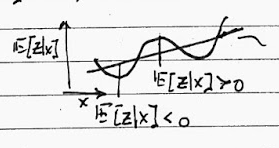
\includegraphics[width=0.4\textwidth]{figures/10-15-1.png}
  \end{center}
\end{figure}

The fact that $\ex[X Z] = 0$ is what gives us the quadratic form representation
for excess loss:
\begin{align}
  L(q, \theta)
  &= \ex_q[(Y - \braket{\theta, X})^2] - \ex_q[(Y - \braket{\theta^*(q), X})^2] \\
  &= \ex_q\left[
    \braket{\theta, X}^2
    + \braket{\theta^*(q), X}^2
    - 2 Y \braket{\theta - \theta^*(q), X}
  \right] \\
  &= \ex_q\left[
    \braket{\theta - \theta^*(q), X}^2
    - 2 \braket{\theta^*(q), X} \braket{X, \theta^*(q) - \theta}
    + 2 Y \braket{X, \theta^*(q) - \theta}
  \right] \\
  &= \ex_q\left[
    \braket{\theta - \theta^*(q), X}^2
    + 2 (Y - \braket{\theta^*(q), X}) \braket{X, \theta^*(q) - \theta}\
  \right] \\
  &= \ex_q\left[
    \braket{\theta - \theta^*(q), X}^2
    + 2 \cancelto{0}{Z \braket{X, \theta^*(q) - \theta}}
  \right] \\
  &= \|\theta - \theta^*(q)\|_{S_q}^2
\end{align}
In this setting, the resilience conditions we need to show are
\begin{itemize}
  \item $\cG_\downarrow$: $\|\theta^*(p) - \theta^*(r)\|_{S_r}^2 \leq \rho$
  \item $\cG_\uparrow$: $\|\theta^*(r) - \theta)\|_{S_r}^2 \leq \rho \implies \|\theta^*(p) - \theta\|_{S_p}^2 \leq 5 \rho$
\end{itemize}
Last time we showed that $\cG_\uparrow$ is implied by
$\cG_\downarrow$ and we took for granted $\|S_r^{-1/2} \ex_r[X Z]\|_2 = \|\ex_r[X Z]\|_{S_r} \leq 2
\sigma \sqrt{\eps}$. This was required for verifying $\cG_\downarrow$ because
by \cref{eq:linreg-second-moment-diff-theta-star}
and \cref{lem:linreg-second-moment-close}
\begin{align}
  \|\theta^*(p) - \theta^*(r)\|_{S_r}^2
  &= \| \ex_r[X Z]\|_{S_r}^2
  \leq 2 \| \ex_r[X Z]\|_{S_p}^2
  = 2 \| S_p^{-1/2} \ex_r[X Z]\|_2^2
\end{align}
The RHS is now just ordinary mean resilience in the $\ell_2$ norm
(note that when $r = p$ the mean is zero), so we can
control it by controlling the covariance and applying
\cref{eg:bdd-cov-resilient}.
By bounding covariance with second moment and using the bounded
noise hypothesis:
\begin{align}
  \Cov_p[S_p^{-1/2} X Z]
  &\leq \ex_p[S_p^{-1/2} X Z^2 X^\top S_p^{-1/2}]
  = S_p^{-1/2} \ex[X Z^2 X^\top] S_p^{-1/2} \\
  &\leq \sigma^2 S_p^{-1/2} \ex[X X^\top] S_p^{-1/2}
  = \sigma^2 I
\end{align}

\subsection{Linear Classification}

Let $(X,Y) \in \RR^d \times \{\pm 1\}$. We can consider the
\emph{classification loss}
\begin{align}
  L(p, \theta) = \Pr_p[Y \neq \sgn\braket{\theta, X}]
\end{align}
or \emph{hinge loss}
\begin{align}
  B(p, \theta) = \ex_{X, y} \max(1 - \braket{\theta, x}y, 0)
\end{align}

\begin{proposition}
  Suppose $p$ satisfies
  \begin{enumerate}
    \item $\ex_{(X,Y) \sim p} \max (1 - y \braket{\theta^*, x}, 0) \leq (1 - \eps) \rho_1$
    \item For all $\theta$ satisfying
      \begin{align}
        \Pr[y \braket{\theta, X} \leq \frac{1}{2}] \leq \eps + 2(1-\eps) \rho_1
      \end{align}
      we have
      \begin{align}
        \Pr[y \braket{\theta, X} \leq 0] \leq \rho_2
      \end{align}
  \end{enumerate}
  Then $p$ is $(\rho_1, \rho-2, \eps)$ resilient.
\end{proposition}
\todo{which loss}?

\begin{proof}
  HW \todo{add when done}
\end{proof}

\begin{remark}
  The second condition is a statement about the rate of tail decay.
  It says that once the tail starts to decay, then it falls off very fast.

  Figure 10.15.XX

  Compare this to bounded variance, which was stronger and required the probability
  mass to be tightly concentrated (i.e.\ tails both fall off very fast and start
  to fall off close to the mean).
\end{remark}

\section{10/17/2019}

\subsection{Efficient Algorithms for Robust Linear Regression}

\begin{itemize}
  \item Last time
    \begin{itemize}
      \item Resilience for linear regression (hypercontractivity and bounded noise)
	and classification (tails decay quickly once they decay at all)
    \end{itemize}
  \item This time
    \begin{itemize}
    	\item Efficient algorithm for linear regression, generalizing previous
	  down-weighting algorithm to filter wrt hypercontractivity and
	  bounded noise
	\item \textbf{Problem}: hypercontractivity is not easy to check.
	  \begin{itemize}
	    \item To work around, replace with stronger condition of
	      ``SoS-certifiably hypercontractive''
	    \item Will need a new SoS tool called ``pseudoexpectations''
	  \end{itemize}
    \end{itemize}
\end{itemize}

\subsection{Pseudoexpectations}

Recall that a sum-of-squares (SoS) program looks like:
\begin{align}
  \max_{y}~& c^\top y  \\
  \text{st}~ p_y(v) &\geq_{SoS} 0~\text{(in $v$)}
\end{align}
where $p_y(v)$ is a polynomial with coefficients linear in $y$.

\begin{definition}[Pseudoexpectation]
  A \emph{degree-2k pseudoexpectation} is a linear map 
  $E : \{\text{degree-$2k$ polynomials}\} \to \RR$ such that
  \begin{enumerate}
    \item $E[1] = 1$
    \item $E[q] \geq 0$ if $q \geq_{SoS} 0$
  \end{enumerate}

  Let $\cE_{2k}$ be the set of all degree-$2k$ pseudoexpectations.
\end{definition}

\begin{remark}
  By linearity and the second property,
  $E[p] \leq E[q]$ if $p \leq_{SoS} q$
\end{remark}

\begin{example}
  $p \mapsto p(v_0)$

  $p \mapsto \ex_{v_0 \sim N(\mu, \Sigma)}[p(v_0)]$
\end{example}

\subsubsection{Efficiency}

\textbf{Question}: Can we efficiently impose a $\cE_{2k}$ constraint?

Yes! Can check membership in this set efficiently
(need to build a \emph{separation oracle}).

To check $E \in \cE_{2k}$
\begin{align}
  \min_q~& E[q] \\
  \text{st}~q &\geq_{SoS} 0\\
  \deg q &\leq 2k
\end{align}
Can parameterize $q$ using $d^{2k}$ coefficients.

\subsubsection{Algorithm}%

\textbf{Setup}: $(X_i, Y_i) \in \RR^d \times \RR$ for $i \in [n]$,
``good'' set $S \subset [n]$ with $\lvert S \rvert = (1 - \eps) n$ of the points.
Think of $p^*$ as uniform on $S$ and $\tilde{p}$ as uniform on $[n]$.

We will be generalizing the bounded covariance algorithm from before.

Need two conditions for our algorithm to work. The first is
\emph{certifiable hypercontractivity}
\begin{align}
  \frac{1}{n}  \sum_{i \in S} \braket{X_i, v}^4 \leq_{SoS} \kappa \left(
    \frac{1}{n} \sum_{i \in S} \braket{X_i, v}^2
  \right)^2
\end{align}
and the second is a generalization of \emph{bounded noise} from before
\begin{align}
  \frac{1}{n} \sum_{i \in S} 
  (\underbrace{Y_i - \braket{\theta^*, X_i}}_{Z_i})^2 X_i X_i^\top
    \preceq \sigma^2 \frac{1}{n} \sum_{i \in S} X_i X_i^\top
\end{align}




\begin{itemize}
  \item \textbf{Input}: $(x_i, y_i)_{i \in [n]}$
  \item \textbf{Initialize}: $c_i = 1$ for all $i \in [n]$
  \item Let $q(\vec{c}) = \sum_{i \in [n]} \frac{c_i}{\sum_i c_i} \delta_{(x_i,
    y_i)}$ be the empirical distribution weighted by $\vec{c}$.
  \item Repeat: $(\hat\theta_c = \argmin_\theta \frac{1}{n}  \sum_{i=1}^n c_i (y_i - \braket{\theta, x_i})^2$
    \begin{itemize}
      \item (check hypercontractivity) Find (if possible) $E \in \cE_{4}$ such that
	\begin{align}
	  E\left[
	    \frac{1}{n} \sum^{n}_{i=1} c_i \braket{x_i, v}^4
	  \right]
	  \geq 3 \kappa E\left[ \left( 
	      \frac{1}{n} \sum^{n}_{i=1} c_i \braket{x_i, v}^2
	  \right)\right]
	\end{align}
      \item If $E$ exists,
	\begin{align}
	  \tau_i &\leftarrow E[\braket{x_i, v}^4]\\
	  c_i &\leftarrow c_i\left(
	    1 - \frac{\tau_i}{\tau_{\max}} 
	  \right)
	\end{align}
	and go to next loop iteration
      \item (check bounded noise) Find (if possible) $v \in \RR^d$ such that
	\begin{align}
	  \frac{1}{n} \sum_{i=1}^n c_i (y_i - \braket{\hat{\theta}_c, x_i})^2 \braket{x_i, v}^2
	  &\geq 24 \sigma^2 \frac{1}{n} \sum^{n}_{i=1} c_i \braket{x_i, v}^2
	\end{align}
      \item If $v$ exists,
	\begin{align}
	  \tau_i &\leftarrow (y_i - \braket{\hat{\theta}_c, x_i})^2 \braket{x_i, v}^2 \\
	  c_i &\leftarrow c_i\left(
	    1 - \frac{\tau_i}{\tau_{\max}} 
	  \right)
	\end{align}
	and go to next loop iteration
    \end{itemize}
  \item Output $\hat{\theta}_c$
\end{itemize}

Each iteration repeatedly finds candidates violating hypercontractivity or
bounded noise and updates $c$ to reduce their influence.

The algorithm is guaranteed to terminate, because some $c_i$ gets set to zero
each iteration so there are at most $n$ iterations.

The following lemma says that $q(c)$ continues to satisfies certifiably
hypercontractive and bounded noise after the updates:
\begin{lemma}
  Suppose $S$ satisfies hypercontractivity and bounded noise conditions,
  and $c_i \in [0,1]$ satisfy $\frac{1}{n}  \sum_{i \in S} (1 - c_i) \leq \eps$.
  Then
  \begin{align}
    \frac{1}{n} \sum_{i \in S} c_i \braket{x_i, v}^4 
    &\leq_{SoS} \frac{\kappa}{1 - \kappa \eps} \left(
      \frac{1}{n} \sum_{i \in S} c_i \braket{x_i, v}^2
    \right)^2 \\
    \frac{1}{n}  \sum_{i \in S} c_i \braket{x_i, v}^2
    &\geq (1 - \kappa \eps) \frac{1}{n}  \sum_{i \in S} \braket{x_i, v}^2
  \end{align}
  The second result implies bounded noise with parameter $\frac{\sigma^2}{1 - \kappa \eps}
  $.
\end{lemma}

\begin{proof}[Proof sketch]
  For the hypercontractivity, if we define 
  \begin{align}
    A &= \frac{1}{n}  \sum_{i \in S} \braket{x_i, v}^4
  \end{align}
  to be the initial distribution for the $4$th moment over $S$
  and 
  \begin{align}
    B &= \frac{1}{n} \sum_{i \in S} \braket{x_i, v}^2
  \end{align}
  and if we define $C$ and $D$ to be the amount we're taking away
  \begin{align}
    C &= \frac{1}{n}  \sum_{i \in S} (1 - c_i) \braket{x_i, v}^4 \\
    D &= \frac{1}{n}  \sum_{i \in S} (1 - c_i) \braket{x_i, v}^2
  \end{align}
  Then we know $\kappa B^2 - A \geq_{SoS} 0$ and 
  $\frac{1}{\eps} c - \left(\frac{1}{\eps} D \right)^2 \geq_{SoS} 0$,
  and we want to show
  \begin{align}
    \frac{\kappa}{1 - \kappa \eps}(B - D)^2 - (A - C)  \geq_{SoS} 0
  \end{align}
  We can check this is true by factoring.
\end{proof}

\begin{proposition}
  If $\eps \leq \frac{1}{100}$ and $\kappa \eps \leq \frac{1}{50}$
  and $q(c)$ satisfies certifiable hypercontractivity and bounded
  noise conditions, then the output of the algorithm has
  excess squared loss $\leq 250 \sigma^2 \eps$.
\end{proposition}

\begin{proof}[Proof structure]
  Same as covariance case:
  \begin{enumerate}
    \item Remove more bad points than good points (so close in $\TV$ distance)
      \begin{align}
	\sum_{i \in S} c_i \tau_i \leq \frac{1}{2} \sum_{i=1}^n c_i \tau_i
      \end{align}
      \begin{itemize}
	\item Hypercontractive 
	\item Bounded noise
      \end{itemize}
    \item $\hat{\theta}_c$ okay if we terminate (use resilience and small $\TV(q(c), p^*)$
  \end{enumerate}

  For hypercontractivity, ``check hypercontractivity''
  filtering step terminates when does not exist pseudoexpectation $E
  \in \cE_4$ refuting hyercontractivity
  \begin{align}
    \frac{1}{n} \sum_{i \in S} c_i E[\braket{x_i, v}^4]
    &\leq \frac{1}{2}  \frac{1}{n}  \sum_{i=1}^n c_i E[\braket{x_i, v}^4] \\
    \frac{1}{n} \sum_{i \in S} c_i E[\braket{x_i, v}^4]
    &\leq \frac{\kappa}{1 - \kappa \eps}  E\left[\left(
	\frac{1}{n}  \sum_{i \in S} c_i \braket{x_i, v}^2
    \right)^2\right] \\
    &\leq \frac{\kappa}{1 - \kappa \eps}  E\left[\left(
	\frac{1}{n}  \sum_{i=1}^n c_i \braket{x_i, v}^2
    \right)^2\right] \\
    \frac{1}{n}  \sum_{i=1}^n c_i E[\braket{x_i, v}^4]
    &\geq 3 \kappa E\left[\left(
	\frac{1}{n} \sum^{n}_{i=1} c_i E[\braket{x_i, v}^2]
    \right)^2\right]
  \end{align}
  so we need $\frac{\kappa}{1 - \kappa \eps} \leq \frac{3 \kappa}{2}$,
  which is true since $\kappa \eps \leq \frac{1}{50}$.

  For bounded noise, need to show
  \begin{align}
    \frac{1}{n} \sum_{i \in S} c_i z_i^2 \braket{x_i, v}^2
    &\leq \frac{1}{2} \frac{1}{n} \sum_{i=1}^n c_i z_i^2 \braket{x_i, v}^2
  \end{align}
  We already have
  \begin{align}
    \braket{x_i, v}^2 \leq 12 \sigma^2 \sum_{i=1}^n c_i \braket{x_i, v}^2
  \end{align}
  and the RHS is lower bounded
  \begin{align}
    \frac{1}{2} \frac{1}{n} \sum_{i=1}^n c_i z_i^2 \braket{x_i, v}^2
    &\geq 24 \sigma^2 \sum_{i=1}^n c_i \braket{x_i, v}^2
  \end{align}
  Expanding $z_i^2$, we have
  \begin{align}
    z_i^2
    &= (y_i - \braket{\hat{\theta}_c, x_i})^2 
    \leq 2 ((y_i - \braket{\theta^*, x_i})^2+ \braket{\hat\theta_c - \theta^*, x_i}^2)
  \end{align}
  the first term has been done and the second is $\leq \frac{\sigma^2}{1 - \kappa -\eps} \frac{1}{n} \sum_{i \in S} c_i \braket{x_i, v}^2$,
  so our goal is to bound
  \begin{align}
    \underbrace{\frac{1}{n}  \sum_{i \in S} \braket{\hat\theta_c - \theta^*, x_i}^2}_{(1-\eps) (\text{excess predictive loss} \coloneqq R)}
    &= \frac{1 - \eps}{\lvert S \rvert} (\theta^* - \hat\theta_c) \underbrace{\sum_{i \in S} x_i x_i^\top}_{\text{second moment matrix}} (\theta^* - \hat\theta_c)
  \end{align}
  By Cauchy-Schwarz and hypercontractivity (applied twice to move back down to $2$nd powers)
  \begin{align}
    \frac{1}{n} \sum_{i \in S} c_i (y_i - \braket{\hat\theta_c, x_i})^2
    &\leq \frac{\sigma^2}{1 - \kappa \eps} \left( \frac{1}{n} \sum_{i \in S} c_i \braket{x_i, v}^2 \right)
    + \frac{1}{n}  \sum_{i \in S} c_i \braket{\hat\theta_c - \theta^*, x_i}^2 \braket{x_i, v}^2
  \end{align}
  Bounding the RHS terms individually
  \begin{align}
    \frac{1}{n}  \sum_{i \in S} c_i \braket{\hat\theta_c - \theta^*, x_i}^2 \braket{x_i, v}^2
    &\leq \sqrt{
      \left(\frac{1}{n} \sum_{i \in S} c_i \braket{\hat\theta_c - \theta^*, x_i}^4\right)
      \left(\frac{1}{n} \sum_{i \in S} c_i \braket{x_i, v}^4\right)
    }\\
    &\leq \frac{\kappa}{1 - \kappa\eps} 
    \underbrace{\left(\frac{1}{n} \sum_{i \in S} c_i \braket{\hat\theta_c - \theta^*, x_i}^2\right)}_{(1 - \eps) R}
      \left(\frac{1}{n} \sum_{i \in S} c_i \braket{x_i, v}^2\right) \\
    \frac{1}{n} \sum_{i \in S} c_i (y_i - \braket{\hat\theta_c, x_i})^2 \braket{x_i, v}^2
    &\leq 
    \underbrace{\left( \frac{\sigma^2}{1 - \kappa \eps} + \frac{(1 - \eps) \kappa R}{1 - \kappa \eps} \right)}_{\leq \sigma^2 / 2}
    \left( \frac{1}{n} \sum_{i \in S} c_i \braket{x_i, v}^2 \right)
  \end{align}

  We can show
  \begin{align}
    R \leq \frac{10 \eps \tilde{\sigma}_c^2}{1 - \eps} 
  \end{align}
  if $\eps \leq \frac{1}{8}$ and $\frac{\eps (\tilde{\kappa} - 1)}{3 \kappa} \leq \frac{1}{6}$.
  So we are happy if
  \begin{align}
    \frac{\sigma^2}{1 - \kappa \eps} + \frac{10 \kappa \eps \tilde{\sigma}^2}{1 - \kappa \eps}
    \leq \frac{\tilde{\sigma}^2}{2} 
  \end{align}
  Doing the algebra, we will find that this holds if $\tilde{\sigma}^2 \geq 256 \sigma^2$.
\end{proof}

\section{10/23/2019 and 10/25/2019}

Was travelling, see course notes for generalizing from $D = \TV$
to Wasserstein distances (need $\eps$-deletion $\to$ $\eps$-``friendly''
and a generalized midpoint lemma).

\section{10/29/2019}

\subsection{Setting for test-time robustness (classification)}
\begin{itemize}
  \item Train: $(x_1, y_1), \ldots, (x_n, y_n) \sim p$,
    $y \in Y$ ($Y = \{\pm 1\}$ binary, $Y = [K]$ multiclass)
  \item Test: $(x, y) \sim p$. Observe $\bar{x}$ such that
    $d(x, \bar{x}) \leq \eps$
    (before $D(\tilde{p}, p^*) \leq \eps$)
  \item Goal: Predict $y$ from $\bar{x}$
\end{itemize}

For various $\ell(\theta; x, y)$, e.g.:
\begin{itemize}
  \item $0/1$-loss, measure accuracy of classifier
  \item log-loss / hinge-loss: measure ``margin'' of classification
\end{itemize}
We were previously using a (non-robust) loss
\begin{align}
  L(p, \theta) &= \ex_{(x,y) \sim p}[ \ell(\theta; x, y) ]
\end{align}
Consider instead a \emph{robust loss}
\begin{align}
  L(p, \theta) &= \ex_{(x,y) \sim p} \left[
    \sup_{\bar{x} : d(x,\bar{x}) \leq \eps} \ell(\theta; \bar{x}, y)
  \right]
\end{align}

We care about this kind of loss because most models are very non-robust
(Figure 10.29.1: a $1/128$ perturbation in $\ell_\infty$
causes a DNN to become very confused)

\subsubsection{Relation to train-time robustness}

Before we thought of the training distribution $\tilde{p}$
as corrupted, and want to ensure performance on the test-time
distribution $p^*$.
Here, we think of the train distribution $p$ as nice and the
test distribution $\bar{p}$ as corrupted.

For classification, we can formalize test-time corruption in terms of
discrepancy as follows:
$D(\tilde{p}, q) \leq \eps$ if there exists a coupling $\pi$ from
$\tilde{p}$ to $q$ such that for $(x,y), (x',y') \sim \pi$
if $y = y'$ then $d(x,x') \leq \eps$ almost surely.

This generalizes Wasserstein distance
\begin{align}
  w_c(p, q) &= \inf_{\pi \in \Pi} \ex_\pi[c(x,x')^k]^{1/k}
\end{align}

Notice here that $\cG$ is not needed.

\subsubsection{Natural algorithm}%

A natural algorithm is to just minimize empirical loss.
For $(x_i, y_i) \simiid p$, fit our model by
\begin{align}
  \min_\theta
  \rho(\theta)
  + \frac{1}{n}  \sum_{i=1}^n
  \sup_{\bar{x}_i : d(x_i, \bar{x}_i) \leq \eps}
  \ell(\theta; \bar{x}_i, y_i)
\end{align}

A couple of issues arise:
\begin{enumerate}
  \item $\sup$ over $\bar{x}$
  \item Generalizataion
  \item What if $d$ wasn't what you cared about?
\end{enumerate}

Some examples of different $d$ we can care about.

Figure 10.29.2

\begin{itemize}
  \item $\ell_\infty$ : each pixel $\leq \eps$
  \item $\ell_1$: total change $\leq \eps$
  \item $\ell_2$
  \item JPEG: $\|JPEG(x) - JPEG(\bar{x})\|_2 \leq \eps$
  \item $\bar{x}$ obtained from $x$ via elastic warping of size $\eps$
  \item Fog
  \item Snow
\end{itemize}

\subsection{Sup over $\bar{x}$}%

The robust loss requires us to compute
\begin{align}
  \sup_{\bar{x} : d(x,\bar{x}) \leq \eps} \ell(\theta; \bar{x}, y)
\end{align}
Unfortunately, $\ell$ is usually not convex in $\bar{x}$
and is hard to optimize.

One strategy is to heuristically maximize $\bar{x}$ by just running a bunch
of gradient steps.
\begin{align}
  \ell_{\text{robust}} &= \sup_{\bar{x}} \ell(\theta; \bar{x}, y) \\
  \ell_{\text{proxy}} &= \text{heuristic max} \\
  \ell_{\text{proxy}} &\leq \ell_{\text{robust}}
\end{align}

This is not a good idea: Figure 10.29.3: minimizing $\theta$ over
the proxy will choose points where the proxy is not a good approximation
to $\ell_{\text{robust}}$








\bibliography{refs.bib}

\end{document}
